\documentclass[12pt,a4paper]{article}
%
%	STARWARE - Stile base per la scrittura di documenti interni in LaTex
%

%
%	Pacchetti globali
%	Fare qui eventuali aggiunte!
%
\usepackage[utf8]{inputenc}
\usepackage[italian]{babel}
\usepackage[babel]{csquotes}
\usepackage{url}
\usepackage{graphicx}
\usepackage[colorlinks]{hyperref}
\usepackage{lastpage}
\usepackage{fancyhdr}
\usepackage[top=1cm,bottom=4cm,left=80pt,right=80pt]{geometry} %disegna la linea
\usepackage{listings} %per grandi porzioni di codice
\usepackage{color}
\usepackage[table]{xcolor}
\usepackage{booktabs,tabularx}
\usepackage{makeidx}
\usepackage{fixltx2e}
\usepackage{hyperref}
\usepackage{enumitem}
\usepackage{color}
\usepackage[T1]{fontenc}
\usepackage{float}
\usepackage{svg}
\usepackage{amsmath}
\usepackage[toc]{glossaries}
\usepackage{dirtree}
\usepackage{listings}

\makeglossaries

\bibliographystyle{alpha}

%
%	VARIABILI GLOBALI
%
\newcommand{\nomeGruppo}{StarWare}
\newcommand{\mailGruppo}{starware.swe@gmail.com}
\newcommand{\uni}{Universit\`{a} degli Studi di Padova}
\newcommand{\uniAA}{2015/2016}
\newcommand{\Cardin}{Prof. Riccardo Cardin}
\newcommand{\Vardanega}{Prof. Tullio Vardanega}
\newcommand{\Zucchetti}{Zucchetti S.p.a.}
\newcommand{\prj}{Quizzipedia}
\newcommand{\prjL}{Quizzipedia: software per la gestione di questionari}

\newcommand{\AVI}{Alessio Vitella}
\newcommand{\AVE}{Andrea Venier}
\newcommand{\NDC}{Nicola De Cao}
\newcommand{\IB}{Igor Baylyak}
\newcommand{\WS}{Walter Sandon}
\newcommand{\TP}{Thomas Pigarelli}
\newcommand{\AB}{Anna Bonaldo}

\newcommand{\mgls}[1]{\gls{#1}\textsubscript{G}}
\newcommand{\mglspl}[1]{\glspl{#1}\textsubscript{G}}
\newcommand{\mGls}[1]{\Gls{#1}\textsubscript{G}}
\newcommand{\mGlspl}[1]{\Glspl{#1}\textsubscript{G}}

\newcommand{\AM}{\emph{\mGls{amministratore}}}
\newcommand{\AN}{\emph{\mGls{analista}}}
\newcommand{\PG}{\emph{\mGls{progettista}}}
\newcommand{\PR}{\emph{\mGls{programmatore}}}
\newcommand{\VR}{\emph{\mGls{verificatore}}}
\newcommand{\PM}{\emph{\mGls{project manager}}}

\newcommand{\AMpl}{\emph{\mGlspl{amministratore}}}
\newcommand{\ANpl}{\emph{\mGlspl{analista}}}
\newcommand{\PGpl}{\emph{\mGlspl{progettista}}}
\newcommand{\PRpl}{\emph{\mGlspl{programmatore}}}
\newcommand{\VRpl}{\emph{\mGlspl{verificatore}}}
\newcommand{\PMpl}{\emph{\mGlspl{project manager}}}

\newcommand{\RR}{\emph{\mGls{revisione dei requisiti}}}
\newcommand{\RA}{\emph{\mGls{revisione di accettazione}}}
\newcommand{\RP}{\emph{\mGls{revisione di progettazione}}}
\newcommand{\RQ}{\emph{\mGls{revisione di qualifica}}}

\newcommand{\NdP}{\emph{\mGls{norme di progetto}}}
\newcommand{\SdF}{\emph{\mGls{stidio di fattibilita}}}
\newcommand{\AdR}{\emph{\mGls{analisi dei requisiti}}}
\newcommand{\PdP}{\emph{\mGls{piano di progetto}}}
\newcommand{\PdQ}{\emph{\mGls{piano di qualifica}}}

\newcommand{\latex}[1]{\texttt{#1}}
\newcommand{\fileName}[1]{\texttt{#1}}
\newcommand{\filePath}[1]{\texttt{#1}}
\newcommand{\TODO}[1]{\texttt{\large \color{red} \underline{TODO: #1}}}

\newcommand{\licenza}{GNU GENERAL PUBLIC LICENSE V2}

%per compilare il template usare questi sotto e commentare glia altri:
%\newcommand{\logoLungo}{../imgs/logoLungo.png}
%\newcommand{\logoGrande}{../imgs/logoGrande.png}
\newcommand{\logoLungo}{../../../template/imgs/logoLungo.png}
\newcommand{\logoGrande}{../../../template/imgs/logoGrande.png}

%
%	Setup stili
%

\newcommand{\HRule}{\rule{\linewidth}{0.5mm}}

\definecolor{dkgreen}{rgb}{0,0.6,0}
\definecolor{gray}{rgb}{0.5,0.5,0.5}
\definecolor{mauve}{rgb}{0.58,0,0.82}
\definecolor{light}{RGB}{255,255,190}

%
%	Setup di pagina
%

%colorazione link
\hypersetup
{
	colorlinks=true,
	linkcolor=black,
	urlcolor=blue,
	citecolor=blue
}

%	Setup Header + Footer

\pagestyle{fancy}
\setlength{\headheight}{2cm} %settato grandezza header

\renewcommand{\footrulewidth}{0.5pt} %ridefinisco il valore della riga di intestazione
\renewcommand{\headrulewidth}{0.5pt} %ridefinisco il valore della riga di pie' di pagina
\addtolength{\headwidth}{\marginparsep}
\addtolength{\headwidth}{\marginparwidth}

\fancyhead{} %annulla head di default
\fancyfoot{} %annulla foot di default

%	Logo intestazione
\lhead{
\includegraphics[scale=0.12]{\logoLungo}}


%	footer
\cfoot{
	\uni \ - \uniAA \\
	\href{mailto:\mailGruppo}{\mailGruppo}\\
	{\tiny Questo documento è distribuito sotto licenza {\licenza}}
}
\rfoot{
	\thepage\ di \pageref{LastPage}
}


% test subsubsubsection

\usepackage{titlesec}
\usepackage{hyperref}

\titleclass{\subsubsubsection}{straight}[\subsection]

\newcounter{subsubsubsection}[subsubsection]
\renewcommand\thesubsubsubsection{\thesubsubsection.\arabic{subsubsubsection}}
\renewcommand\theparagraph{\thesubsubsubsection.\arabic{paragraph}} % optional; useful if paragraphs are to be numbered

\titleformat{\subsubsubsection}
  {\normalfont\normalsize\bfseries}{\thesubsubsubsection}{1em}{}
\titlespacing*{\subsubsubsection}
{0pt}{3.25ex plus 1ex minus .2ex}{1.5ex plus .2ex}

\makeatletter
\renewcommand\paragraph{\@startsection{paragraph}{5}{\z@}%
  {3.25ex \@plus1ex \@minus.2ex}%
  {-1em}%
  {\normalfont\normalsize\bfseries}}
\renewcommand\subparagraph{\@startsection{subparagraph}{6}{\parindent}%
  {3.25ex \@plus1ex \@minus .2ex}%
  {-1em}%
  {\normalfont\normalsize\bfseries}}
\def\toclevel@subsubsubsection{4}
\def\toclevel@paragraph{5}
\def\toclevel@paragraph{6}
\def\l@subsubsubsection{\@dottedtocline{4}{7em}{4em}}
\def\l@paragraph{\@dottedtocline{5}{10em}{5em}}
\def\l@subparagraph{\@dottedtocline{6}{14em}{6em}}
\makeatother

\setcounter{secnumdepth}{4}
\setcounter{tocdepth}{4}


%pdflatex -synctex=1 -interaction=nonstopmode %.tex|makeglossaries %|pdflatex -synctex=1 -interaction=nonstopmode %.tex|pdflatex -synctex=1 -interaction=nonstopmode %.tex
\makeglossary

\newglossaryentry{responsabile} {
	name=responsabile,
	description={è il responsabile della gestione, pianificazione e realizzazione del progetto},
	plural=Responsabili
}

\newglossaryentry{verificatore} {
	name=verificatore,
	description={è il responsabile dell'attività di verifica},
	plural=Verificatori
}

\newglossaryentry{programmatore} {
	name=programmatore,
	description={è responsabile delle attività di codifica miranti alla realizzazione del prodotto e delle componenti di ausilio necessarie per l'esecuzione delle prove di verifica e validazione},
	plural=programmatori
}

\newglossaryentry{progettista} {
	name=progettista,
	description={è responsabile delle attività di progettazione},
	plural=Progettisti
}

\newglossaryentry{analista} {
	name=analista,
	description={è responsabile delle attività di analisi. },
	plural=Analisti
}

\newglossaryentry{amministratore} {
	name=amministratore,
	description={è responsabile dell'efficienza e dell'operatività dell'ambiente di sviluppo; si occupa della redazione e attuazione di piani e procedure di gestione della qualità; inoltre gestisce l'archivio della documentazione del progetto},
	plural=Amministratori
}

\newglossaryentry{revisione dei requisiti} {
	name=revisione dei requisiti,
	description={è una revisione formale che determina l'accesso del gruppo al progetto didattico e la concordanza con il cliente di una visione condivisa del prodotto atteso}
}

\newglossaryentry{revisione di accettazione} {
	name=revisione di accettazione,
	description={è una revisione formale per l'accertamento del soddisfacimento di tutti i requisiti e il completamento del progetto}
}

\newglossaryentry{revisione di progettazione} {
	name=revisione di progettazione,
	description={è una revisione di progresso che accerta la realizzabilità del prodotto e informa il cliente sulle caratteristiche del prodotto}
}

\newglossaryentry{revisione di qualifica} {
	name=revisione di qualifica,
	description={è una revisione di progresso che approva l'esito finale delle verifiche e attiva la fase di validazione}
}

\newglossaryentry{analisi} {
	name=analisi,
	description={è il periodo di preparazione e produzioni di documenti che precede la Revisione dei requisiti}
}

\newglossaryentry{progettazione} {
	name=progettazione,
	description={è il periodo che intercorre tra la Revisione dei requisiti e la Revisione di progettazione}
}

\newglossaryentry{codifica} {
	name=codifica,
	description={è il periodo che intercorre tra la Revisione di progettazione e la Revisione di qualifica}
}

\newglossaryentry{validazione} {
	name=validazione,
	description={è il periodo che intercorre tra la Revisione di qualifica e la Revisione di accettazione}
}

\newglossaryentry{repository} {
	name=repository,
	description={è dove i file sono memorizzati, spesso su un server}
}

\newglossaryentry{ruolo} {
	name=ruolo,
	description={una delle figure professionali che una persona fisica interpreta nel corso del progetto. I ruoli sono: responsabile, amministratore, analista, progettista, programmatore e verificatore},
    plural=ruoli
}

\newglossaryentry{svg} {
	name=SVG,
	description={è un formato per la visualizzazione di oggetti in grafica vettoriale. Per maggiori informazioni si veda \href{https://it.wikipedia.org/wiki/Scalable_Vector_Graphics}{qui}}
}

\newglossaryentry{png} {
	name=PNG,
	description={abbreviazione di Portable Network Graphics, è un formato di file per memorizzare immagini. Per ulteriori informazioni si veda \href{http://it.wikipedia.org/wiki/Portable_Network_Graphics}{qui}}
}

\newglossaryentry{pdf} {
	name=PDF,
	description={è un formato di file basato su un linguaggio di descrizione di pagina sviluppato da Adobe Systems nel 1993 per rappresentare documenti in modo indipendente dall’hardware e dal software utilizzati per generarli o per visualizzarli. Per ulteriori informazioni si veda \href{http://it.wikipedia.org/wiki/Portable_Document_Format}{qui}}
}

\newglossaryentry{uml} {
	name=UML,
	description={è un linguaggio di modellazione e specifica basato sul paradigma object-oriented. Per ulteriori informazioni si veda \href{http://it.wikipedia.org/wiki/Unified_Modeling_Language}{qui}}
}

\newglossaryentry{walkthrough} {
	name=walkthrough,
    description={consiste nella lettura di un documento o codice cercando errori ed anomalie senza un'idea precisa di quali tipi di errori sarà possibile trovare}
}

\newglossaryentry{lista di controllo} {
	name=lista di controllo,
	description={è un elenco di cose da fare per eseguire una determinata attività}
}

\newglossaryentry{inspection} {
	name=inspection,
	description={è la lettura mirata di un documento o codice cercando errori specifici}
}

\newglossaryentry{milestone} {
	name=milestone,
	description={momento saliente nello sviluppo di un prodotto software per la quale devono essere pronti documenti e/o funzionalità}
}

\newglossaryentry{ticket} {
	name=ticket,
	description={rappresenta un compito nell'organizzazione e distribuzione del lavoro all'interno del progetto},
	plural=tickets
}

\newglossaryentry{commit} {
	name=commit,
	description={è la copia di modifiche fatte su file locali verso la repository remota. Esso rappresenta anche un particolare stato della repository nel tempo}
}

\newglossaryentry{versionamento} {
	name=versionamento,
	description={è la gestione di un versioni multiple di un insieme di informazioni. Per maggiori informazioni si veda \href{http://it. wikipedia.org/wiki/Controllo_versione}{qui}}
}

\newglossaryentry{task} {
	name=task,
	description={è un compito secondo la definizione dello standard IEEE 12207},
	plural=tasks
}

\newglossaryentry{attivita} {
	name=attivita,
	description={è un insieme di task}
}

\newglossaryentry{redattore} {
	name=redattore,
	description={colui che redige un documento},
	plural=redattori
}

\newglossaryentry{proponente} {
	name=proponente,
	description={colui che ha proposto al committente un capitolato d'appalto}
}

\newglossaryentry{committente} {
	name=committente,
	description={colui che assegna un compito. In questo caso è il Professor Tullio Vardanega}
}

\newglossaryentry{quality assurance} {
	name=quality assurance,
	description={è l'insieme delle attività volte a garantire il soddisfacimento degli obiettivi della qualità}
}

\newglossaryentry{telegram} {
	name=telegram,
	description={è un servizio di messaggistica istantanea utilizzato dal gruppo per comunicazioni interne. Per maggiori informazioni si veda \href{https://it.wikipedia.org/wiki/Telegram_(software)}{qui}}
}

\newglossaryentry{browser} {
	name=browser,
	description={è un'applicazione per il recupero, la presentazione e la navigazione di risorse web}
}

\newglossaryentry{google drive} {
	name=Google Drive,
	description={è un servizio di memorizzazione e sincronizzazione online introdotto da Google il 24 aprile 2012. Per maggiori informazioni si veda \href{https://it.wikipedia.org/wiki/Google_Drive}{qui}}
}

\newglossaryentry{skype} {
	name=Skype,
	description={è un software proprietario freeware di messaggistica istantanea e VoIP. Per maggiori informazioni si veda \href{https://it.wikipedia.org/wiki/Skype}{qui}}
}

\newglossaryentry{gantt} {
	name=Gantt,
	description={è un diagramma di supporto alla gestione dei progetti}
}

\newglossaryentry{projectlibre} {
	name=ProjectLibre,
	description={è un software di gestione progettuale}
}

\newglossaryentry{pert} {
	name=PERT,
	description={è uno strumento volto alla programmazione delle attività che compongono il progetto e, più in generale, alla gestione degli aspetti temporali di quest'ultimo}
}

\newglossaryentry{subtask} {
	name=subtask,
	description={è un task compreso all'interno di un altro task. La totalità di tutti i subtasks costituisce un intero task}
	plural=subtasks
}

\newglossaryentry{ticketing} {
	name=ticketing,
	description={procedura con la quale il Responsabile assegna un task}
}

\newglossaryentry{git} {
	name=git,
	description={è un sistema software di controllo di versione distribuito}
}

\newglossaryentry{quizzpedia} {
	name=Quizzpedia,
	description={è il nome del prodotto software richiesto dal capitolato d'appalto scelto}
}

\newglossaryentry{schierabile} {
	name=schierabile,
	description={è la capacità di rilasciare al cliente, con relativa installazione e messa in funzione o esercizio, di una applicazione o di un sistema software tipicamente all'interno di un sistema informatico aziendale}
}

\newglossaryentry{cross-platform} {
	name=cross-platform,
	description={può essere riferito ad un linguaggio di programmazione, ad un'applicazione software o ad un dispositivo hardware che funziona su più di un sistema}
}

\newglossaryentry{qml} {
	name=QML,
	description={è un "Domain Specific Language" richiesto dal capitolato d'appalto per la definizione delle domande all'interno del sistema}
}

\newglossaryentry{tomcat} {
	name=Tomcat,
	description={è un application server nella forma di contenitore servlet open source sviluppato dalla Apache Software Foundation. Per maggiori informazioni si veda \href{https://it.wikipedia.org/wiki/Apache_Tomcat}{qui}}
}

\newglossaryentry{java} {
	name=Java,
	description={è un linguaggio di programmazione orientato agli oggetti, specificatamente progettato per essere il più possibile indipendente dalla piattaforma di esecuzione. Per maggiori informazioni si veda \href{https://it.wikipedia.org/wiki/Java_(linguaggio_di_programmazione)}{qui}}
}

\newglossaryentry{node.js} {
	name=Node.js,
	description={è un framework che permette di realizzare web application usando un linguaggio di programmazione che utilizza la stessa sintassi di JavaScrip. Utilizza un modello event-driven, anzichè il classico modello a processi o thread concorrenti, e ciò significa che si eseguono azioni solo al verificarsi di un evento. Questo modello asincrono rende leggero ed efficiente, ideale per applicazioni real-time in per dispositivi distribuiti}
}

\newglossaryentry{javascript} {
	name=JavaScript,
	description={linguaggio di scripting orientato agli oggetti comunemente usato nella programmazione
Web}
}

\newglossaryentry{postgresql} {
	name=PostgreSQL,
	description={e un sistema di gestione di basi di dati open source usato per applicazioni che richiedono caratteristiche molto complesse complesse}
}

\newglossaryentry{mongodb} {
	name=MongoDB,
	description={è un sistema gestionale di basi di dati NoSQL orientato ai documenti, adatto per ambienti che hanno la necessità d'immagazzinare grosse quantità di dati, e dove il linguaggio utilizzato per la gestione dei dati è \mgls{javascript}}
}

\newglossaryentry{html5} {
	name=HTML5,
	description={linguaggio di markup per la strutturazione delle pagine web}
}

\newglossaryentry{css3} {
	name=CSS3,
	description={è un linguaggio di programmazione web utilizzato per descrivere l'aspetto e la formattazione di un sito web al browser lato client. }
}

\newglossaryentry{xml} {
	name=XML,
	description={è un meta-linguaggio che fornisce un insieme standard di regole sintattiche per modellare la struttura di documenti e dati. Questo insieme di regole, definiscono le modalità secondo cui è possibile crearsi un proprio linguaggio di markup}
}

\newglossaryentry{nosql} {
	name=NoSQL,
	description={come dice anche il termine questi database non sono basati su SQL, non sono basati su uno schema relazionale. I database relazionali sono infatti ottimi quando esistono delle relazioni tra i dati che salviamo, ma sono poco performanti nel caso sia necessario salvare una grande quantità di dati, magari usando la scalabilità orizzontale, quando cioè si utilizzano più server dove salvare questi dati e non solamente incrementando la potenza di un singolo server.
}
}

\newglossaryentry{scala} {
	name=Scala,
	description={è un linguaggio di programmazione di tipo general-purpose multi-paradigma studiato per integrare le caratteristiche e funzionalità dei linguaggi orientati agli oggetti e dei linguaggi funzionali. Per maggiori informazioni si veda \href{https://it.wikipedia.org/wiki/Scala_(linguaggio_di_programmazione)}{qui}}
}

\newglossaryentry{akka} {
	name=Akka,
	description={è un toolkit di strumenti per la costruzione di applicazioni con elevata concorrenza di dati che necessitano di un sistema resilente per l'invio e la ricezione di messaggi}
}

\newglossaryentry{ble} {
	name=BLE,
	description={Bluetooth low energy,  pur mantenendo un range di comunicazione simile a quello classico, fornisce un  consumo energetico dei device notevolmente ridotto}
}

\newglossaryentry{mqtt} {
	name=MQTT,
	description={è un protocollo di messaggistica leggero posizionato in cima a TCP/IP, disegnato per le situazioni in cui è richiesto un basso impatto e dove la banda è limitata. }
}

\newglossaryentry{aws} {
	name=AWS,
	description={è un insieme di servizi di elaborazione rermoti, detti anche servizi web, che costituiscono una piattaforma di cloud computing offerto da Amazon. Per maggiori informazioni si veda \href{https://aws.amazon.com/it/}{qui}}
}

\newglossaryentry{heroku} {
	name=Heroku,
	description={è una  delle prime cloud Platform-as-a-Service (PaaS) che supportava solo Java come linguaggio di programmazione, oggi giorno ha aggiunto molti altri linguaggi come Scala, Phyton, etc. Per maggiori informazioni si veda \href{https://www.heroku.com}{qui}}
}

\newglossaryentry{github} {
	name=Github,
	description={software di controllo di versione che permette di aggiornare un file senza dover sovrascrivere le versioni precedenti}
}

\newglossaryentry{template} {
	name=template,
	description={traducibile in italiano come modello, indica o un programma o un documento idealizzato come un documento semicompilato cartaceo che ha degli spazi bianchi che saranno successivamente riempiti}
	plural=templates
}

\newglossaryentry{dropbox} {
	name=Dropbox,
	description={è un software di cloud storage multipiattaforma, che offre un servizio di file hosting e sincronizzazione automatica di file tramite web}
}

\newglossaryentry{open-source} {
	name=open-source,
	description={un software di cui gli autori ovvero i detentori dei diritti rendono pubblico il codice sorgente, favorendone il libero studio e permettendo a programmatori indipendenti di apportarvi modifiche ed estensioni. Questo è realizzato tramite apposite licenze d'uso}
}

\newglossaryentry{project management} {
	name=project management,
	description={si intende l'insieme di attività aziendali, svolte tipicamene da una figura dedicata e specializzata detta project manager, volte all'analisi, progettazione, pianificazione e realizzazione degli obiettivi di un progetto, gestendolo in tutte le sue caratteristiche e fasi evolutive, nel rispetto di precisi vincoli come i tempi, costi, risorse, scopi, qualità}
}

\newglossaryentry{linux} {
	name=Linux,
	description={è una famiglia di sistemi operativi open-source di tipo Unix-like, rilasciati sotto varie possibili distribuzioni, aventi la caratteristica comune di utilizzare come nucleo il kernel Linux}
}

\newglossaryentry{windows} {
	name=Windows,
	description={è una famiglia di ambienti operativi e sistemi operativi dedicati ai personal computer, alle workstation, ai server e agli smartphone. Il sistema operativo si chiama così per via della sua interfaccia di programmazione di un'applicazione a finestre}
}

\newglossaryentry{mac os} {
	name=Mac OS,
	description={il sistema operativo di Apple dedicato dedicati ai personal computer Macintosh, alle workstation, ai server e agli smartphone  }
}


\newglossaryentry{schedule variance} {
	name=schedule variance,
	description={ogni deviazione alle baseline di un progetto, misurata confrontando costo preventivato di programma di lavoro con il costo preventivato del lavoro svolto. Indica quindi al cliente se il progetto sta procedendo nei tempi stabiliti}
}

\newglossaryentry{cost variance} {
	name=cost variance,
	description={indica al management aziendale se il valore del costo realmente maturato è maggiore, uguale o minore rispetto al costo pianificato}
}


\newglossaryentry{merge} {
	name=merge,
	description={unire due o più quantità}
}

\newglossaryentry{slack} {
	name=slack,
	description={intervallo di tempo entro cui un evento deve avvenire nel rispetto dei vincoli logici e imposti dal reticolo di pianificazione senza compromettere la durata complessiva del progetto}
}

\newglossaryentry{baseline} {
	name=baseline,
	description={di progetto costituisce il punto di riferimento rispetto al quale calcolare gli scostamenti delle principali variabili implicate nella gestione di un progetto}
}

\newglossaryentry{asana} {
	name=Asana,
	description={è un software che permette a dei team di monitorare il loro lavoro e tener traccia dei risultati tramite l'assegnazione di task a componemti specifiche del gruppo di lavoro}
}

\newglossaryentry{deadline} {
	name=deadline,
	description={La deadline di un \mgls{task} è un indicazione dell'urgenza del \mgls{task}; rappresenta un un punto su una linea temporale ideale. Data di scadenza o termine entro il quale deve essere completato un compito assegnato.}
}

\newglossaryentry{revert} {
	name=revert,
	description={per annullare le ultime modifiche effettuate al repository remoto. Per maggiori informazioni si veda \href{https://git-scm.com/docs/}{qui}}
}

\newglossaryentry{backup} {
	name=backup,
	description={si indica la replicazione, su un qualunque supporto di memorizzazione, di materiale informativo archiviato nella memoria di massa, al fine di prevenire la perdita definitiva dei dati in caso di eventi malevoli accidentali o intenzionali}
}

\newglossaryentry{push} {
	name=push,
	description={per inviare modifiche di un documento site in un host locale al repository remoto. Per maggiori informazioni si veda \href{https://git-scm.com/docs/}{qui}}
}

\newglossaryentry{teamwork} {
	name=teamwork,
	description={è un software che permette a dei team di monitorare il loro lavoro e tener traccia dei risultati tramite l'assegnazione di task a componenti specifiche del gruppo di lavoro}
}

\newglossaryentry{evento} {
	name=evento,
	description={\mgls{teamwork}, attraverso il suo calendario, offre la possibilità di impostare eventi in giorni stabiliti dagli utenti. Questi eventi verranno periodicamente segnalati come promemoria a tutte le persone invitate agli stessi.}
}

\newglossaryentry{etichetta} {
	name=etichetta,
	description={è un controllo grafico che mostra informazioni testuali all'interno di un form}
	plural=etichette
}

\newglossaryentry{bug} {
	name=bug,
	description={identifica un errore nella scrittura di un programma software che ne causa un comportamento imprevisto o comunque diverso da quello specificato dal produttore}
	plural=bugs
}

\newglossaryentry{software} {
	name=software,
	description={e’ un termine generico che definisce programmi e procedure utilizzati per far eseguire al computer un determinato compito}
}

\newglossaryentry{desktop} {
	name=desktop,
	description={area dello schermo su cui appaiono le icone e le finestre rappresentanti le memorie di massa collegate al computer ed il loro contenuto}
}

\newglossaryentry{draw.io} {
	name=draw.io,
	description={é un software gratuito per la creazione di diagrammi di flusso, di processo, UML, e diagrammi di rete}
}

\newglossaryentry{tracy} {
	name=tracy,
	description={software opensource per il tracciamento}
}

\newglossaryentry{package} {
	name=package,
	description={è un meccanismo per organizzare classi Java in gruppi logici, principalmente allo scopo di definire namespace distinti per diversi contesti}
}

\newglossaryentry{stakeholder} {
	name=stakeholder,
	description={si indica genericamente un soggetto o un gruppo di soggetti influenti nei confronti di un'iniziativa economica, sia essa un'azienda o un progetto}
}

\newglossaryentry{branch} {
	name=branch,
	description={quando si vuole creare un nuovo ramo al repository remoto. Per maggiori informazioni si veda \href{https://git-scm.com/docs/}{qui}}
	plural=branches
}

\newglossaryentry{pull} {
	name=pull,
	description={un comando gitub per poter ricevere nell'host locale tutte le modifiche fatte nel repository remoto. Per maggiori informazioni si veda \href{https://git-scm.com/docs/}{qui}}
}

\newglossaryentry{underscore} {
	name=underscore,
	description={è un carattere che identifica il trattino basso}
}

\newglossaryentry{spelling} {
	name=spelling,
	description={è l'atto di pronunciare le parole lentamente, separando le singole lettere o le sillabe}
}

\newglossaryentry{cloud} {
	name=cloud,
	description={si indica un sistema di erogazione di risorse informatiche, come l'archiviazione, l'elaborazione o la trasmissione di dati, caratterizzato dalla disponibilità on demand attraverso Internet}
}

\newglossaryentry{smartphone} {
	name=smartphone,
	description={è un telefono cellulare con capacità di calcolo, di memoria e di connessione dati molto più avanzate rispetto ai normali telefoni cellulari}
	plural=smartphones
}

\newglossaryentry{checkbox} {
	name=checkbox,
	description={è un controllo grafico con cui l'utente può effettuare selezioni multiple}
}


\newglossaryentry{makefile} {
	name=makefile,
	description={è usata soprattutto per la compilazione di codice sorgente in codice oggetto, unendo e poi linkando il codice oggetto in programmi eseguibili o in librerie}
}

\newglossaryentry{gulpease} {
	name=Gulpease,
	description={è un indice di leggibilità di un testo tarato sulla lingua italiana. Rispetto ad altri ha il vantaggio di utilizzare la lunghezza delle parole in lettere anziché in sillabe, semplificandone il calcolo automatico}
}

\newglossaryentry{pdca} {
	name=PDCA,
	description={\TODO{}}
}

\usepackage{verbatim}
%Titolo documento
\newcommand{\titoloDocumento}{Manuale Utente}

%Prima data di creazione del documento
\newcommand{\dataCreazione}{26 aprile 2016}

%Inserite la versione attuale del documento
\newcommand{\versione}{0.0.0}

%Stato in cui si trova il documento: Formale solo all'atto di consegna
\newcommand{\stato}{Formale}

%Uso del documento
\newcommand{\uso}{Esterno}

\rhead{\titoloDocumento}
\lfoot{Versione: \versione}
\title{\titoloDocumento}

\begin{document}
	\begin{titlepage}
		\begin{center}
			\intestazione{\titoloDocumento}
			
			\begin{table}[h]
				\begin{center}
					\begin{tabular}{r | l}
						\multicolumn{2}{c}{\textbf{Informazioni sul documento}}\\
						\midrule
						\textbf{Nome Documento}	&	\titoloDocumento	\\
						\textbf{Versione}	&	\versione	\\
						\textbf{Stato}	&	\emph{\stato}	\\
						\textbf{Uso}	&	\emph{\uso}	\\
						\textbf{Data Creazione}	&	\dataCreazione	\\
						\textbf{Data Ultima Modifica}	&	\today	\\
						\textbf{Redazione}	\\
						\textbf{Verifica}	&		\\
						\textbf{Approvazione}	& \AB{} \\
						\textbf{Lista distribuzione}	&	\nomeGruppo{}	\\
						\ 	&	\Vardanega{}	\\
						\ 	&	\Cardin{}	\\
						\ 	&	Il \mgls{proponente} \Zucchetti{}	\\
						
					\end{tabular}
				\end{center}
			\end{table}
			
		\end{center}
	\end{titlepage}
	\newpage
	
	\Large{\textbf{Registro delle modifiche}}\\
	\normalsize
	
	\begin{center}
		\begin{longtable}[H]{p{0.12\textwidth} p{0.2\textwidth} p{0.18\textwidth} p{0.39\textwidth}}
			\toprule
			\textbf{Versione}	&	\textbf{Autore}	&	\textbf{Data}	&	\textbf{Descrizione}\\*
			\midrule
			0.0.2 & \WS{} & 2016-05-10 &  Correzioni al documento ed inserimento screenshot \\*
			\midrule
			0.0.1 & \WS{} & 2016-05-09 &  Inserimento sezione amministratore e proprietario \\*
			\midrule
			0.0.0 & \AB{} & 2016-04-26 &  Creazione documento \\*
			\bottomrule
			\caption{\mGls{versionamento}  del documento}
			\label{tabVers1}
		\end{longtable}
	\end{center}
	
	\newpage
	\tableofcontents
	\newpage
	\listoftables
	\listoffigures
	\newpage
	
	
	\section{Introduzione}	\label{intro}
	
	\subsection{Scopo}
	Lo scopo del seguente documento è fornire una guida dettagliata all’utente per l’utilizzo dell’applicazione \prj{}. Sono descritte le funzionalità dell'applicazione e i profili utente offerti.
	Vengono inoltre specificati i requisiti tecnici per l'utilizzo dell'applicazione \prj{}.

	\subsection{Descrizione}
    Il documento include la descrizione dettagliata delle funzionalità offerte dal sistema per ogni tipo di utente previsto. In particolar modo, vengono definite tutte le funzionalità offerte dal sistema all’utente con l’ausilio di immagini illustrative. 
    I requisiti tecnici per l'utilizzo dell'applicazione \prj{} sono specificati nel dettaglio.
	
	\subsection{Descrizione Prodotto}
	\descrizioneProdotto
	
	\subsection{Glossario}
	\glossarioPrint
	\subsection{Comunicazione malfunzionamenti}
	Se durante l’utilizzo dell’applicazione Quizzipedia si dovessero riscontrare problemi o
	malfunzionamenti, si invitano gli utilizzatori a segnalare l’errore inviando una email all’indirizzo:
	\url{starware.swe@gmail.com}
	Nella mail di segnalazione si dovranno riportare:
	\begin{itemize}
		\item \mgls{username} fornito in fase di registrazione dell’applicazione (ATTENZIONE: non è richiesta la password di autenticazione);
		\item versione di browser e sistema operativo utilizzato. Nel caso di dispositivi mobile il modello utilizzato;
		\item descrizione dettagliata del problema riscontrato e relativi errori visualizzati;
	\end{itemize}
	Prima di aprire una richiesta di assistenza si consiglia di effettuare operazioni di pulizia dei file \mglspl{cookie}. Per le istruzioni fare riferimento alle specifiche funzionali di ciascun \mgls{browser}.
	
	\subsection{Riferimenti}
	
\subsubsection{Normativi}
\begin{itemize}
	\item \NdP\ \textit{v1.2.0};
	\item Capitolato d'appalto C5: \url{http://www.math.unipd.it/~tullio/IS-1/2015/Progetto/C5p.pdf}.
\end{itemize}

	
	\newpage
	\section{Requisiti per l'utilizzo dell'applicazione} 
	\subsection{Requisiti hardware}
	Per poter utilizzare l'applicazione \prj{} è necessario:
	\begin{itemize}
		\item disporre di una connessione internet;
	\end{itemize}
	\subsection{Requisiti software}
	
	Affinché l’applicazione possa funzionare correttamente tramite computer \mgls{desktop} è necessario disporre di uno dei seguenti \mgls{browser}:
	\begin{itemize}
		\item \textit{\textbf{Google Chrome}}: versione  47.0.2526 o superiore
		\item \textit{\textbf{Microsoft Edge}}: versione 25.10586 o superiore
	\item \textit{\textbf{Mozilla Firefox}}: versione 38.5.2esr o superiore
	\item\textit{\textbf{Safari}}: versione 9.0.2 o superiore
	\end{itemize}
	Il browser deve avere necessariamente Javascript abilitato.\\
	
 L'applicazione è supportata sui seguenti dispositivi mobile:
	\begin{itemize}
	\item \textit{\textbf{Android}} dalla versione 4.0
	\item \textit{\textbf{iOS}} dalla versione iOS6
\end{itemize}

	\newpage
	\section{Autenticazione e gestione profilo}
	\subsection{Registrazione}\label{registrazione}
	Per accedere all'applicazione la prima volta è necessario effettuare la registrazione. Nel caso si sia già effettuata questa procedura una volta, si veda la sezione \ref{autenticazione}.
	Per effettuare la procedura di registrazione è necessario:
	\begin{itemize}
		\item inserire l'\mgls{username};
		\item inserire nome completo;
		\item inserire la password;
		\item ripetere la password;
		\item selezionare il pultasante "SUBMIT". 
	\end{itemize}

\begin{figure}[h]
		
\centering
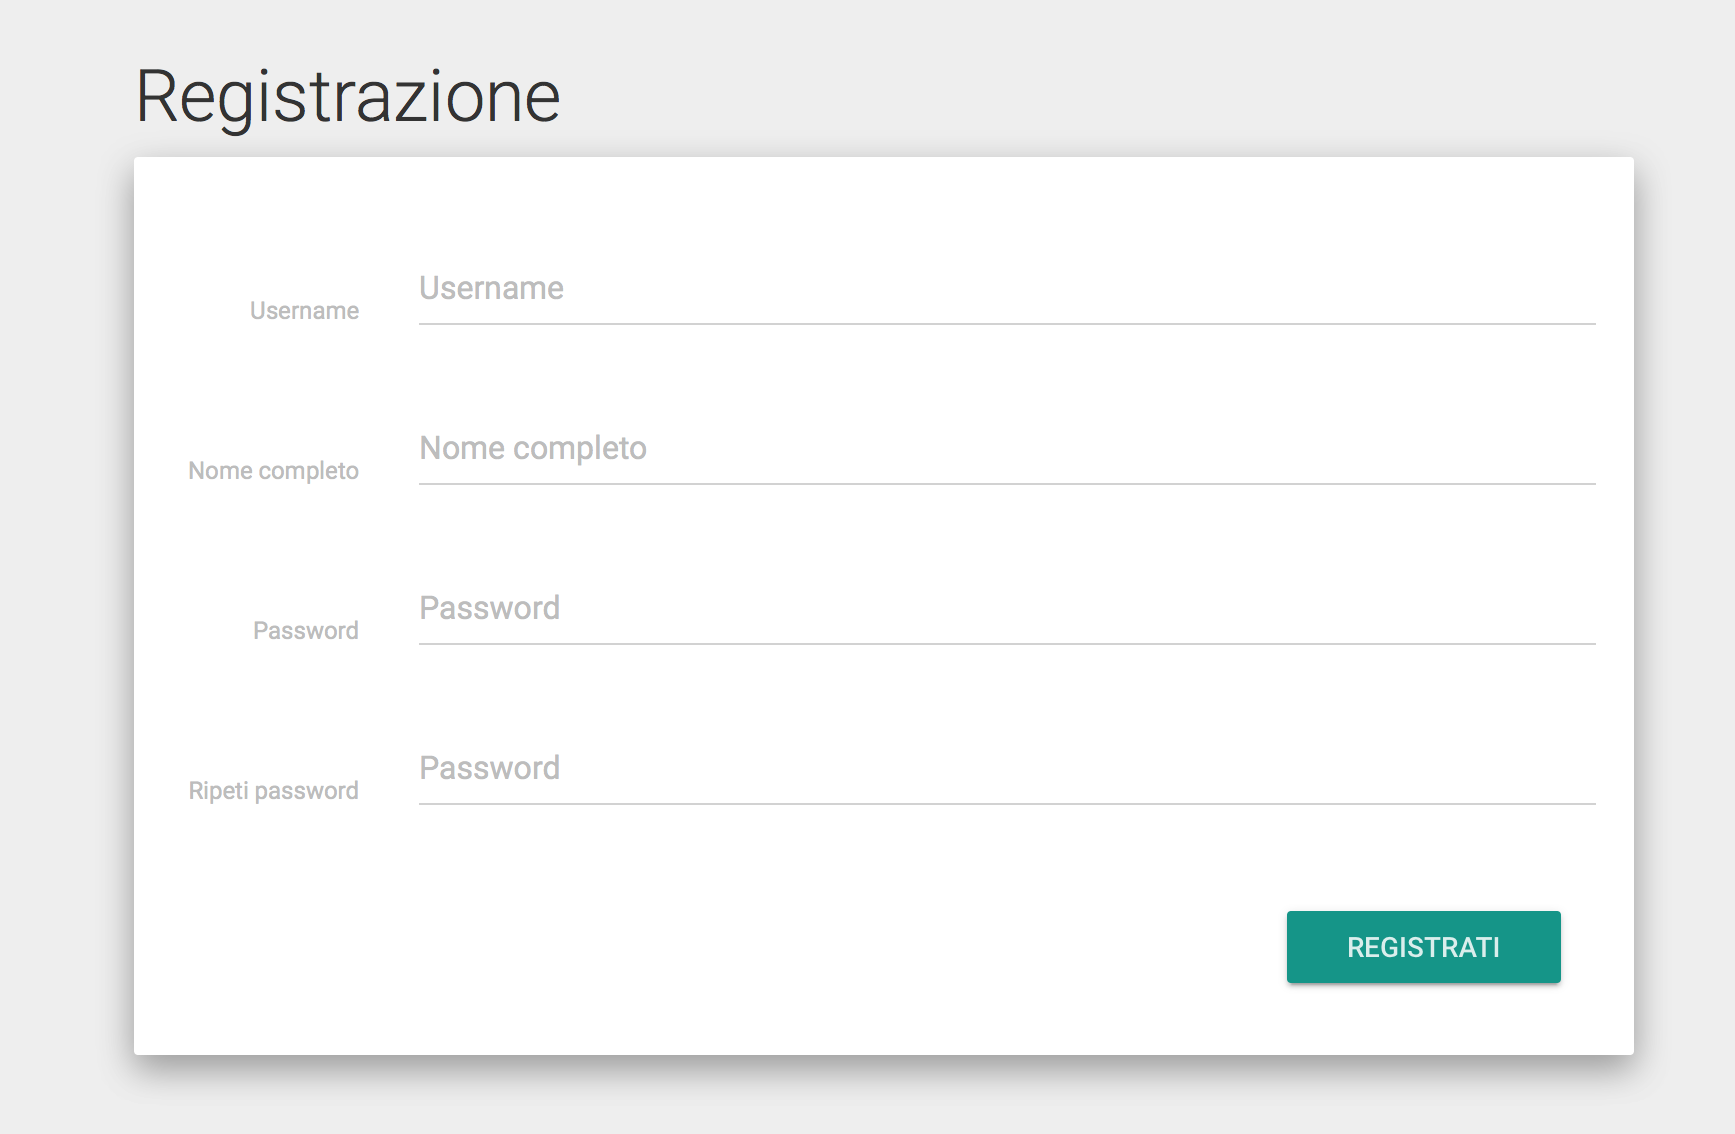
\includegraphics[width=0.8\linewidth]{../img/screenshot/signup.png}
\caption{}
\label{Schermata di registrazione}
\end{figure}


	\subsection{Autenticazione}\label{autenticazione}
	Per accedere alle funzionalità dell'applicazione è necessario effettuare l'autenticazione. Nel caso non si posseggano le credenziali di accesso si veda la sezione di \ref{registrazione}.
	Per effettuare l'autenticazione è necessario:
	\begin{itemize}
		\item inserire l'\mgls{username} corretto;
		\item inserire la password corrispondente corretta;
		\item selezionare il pulsante "SUBMIT".
	\end{itemize}
	
		\begin{figure}[h]
		
		\centering
		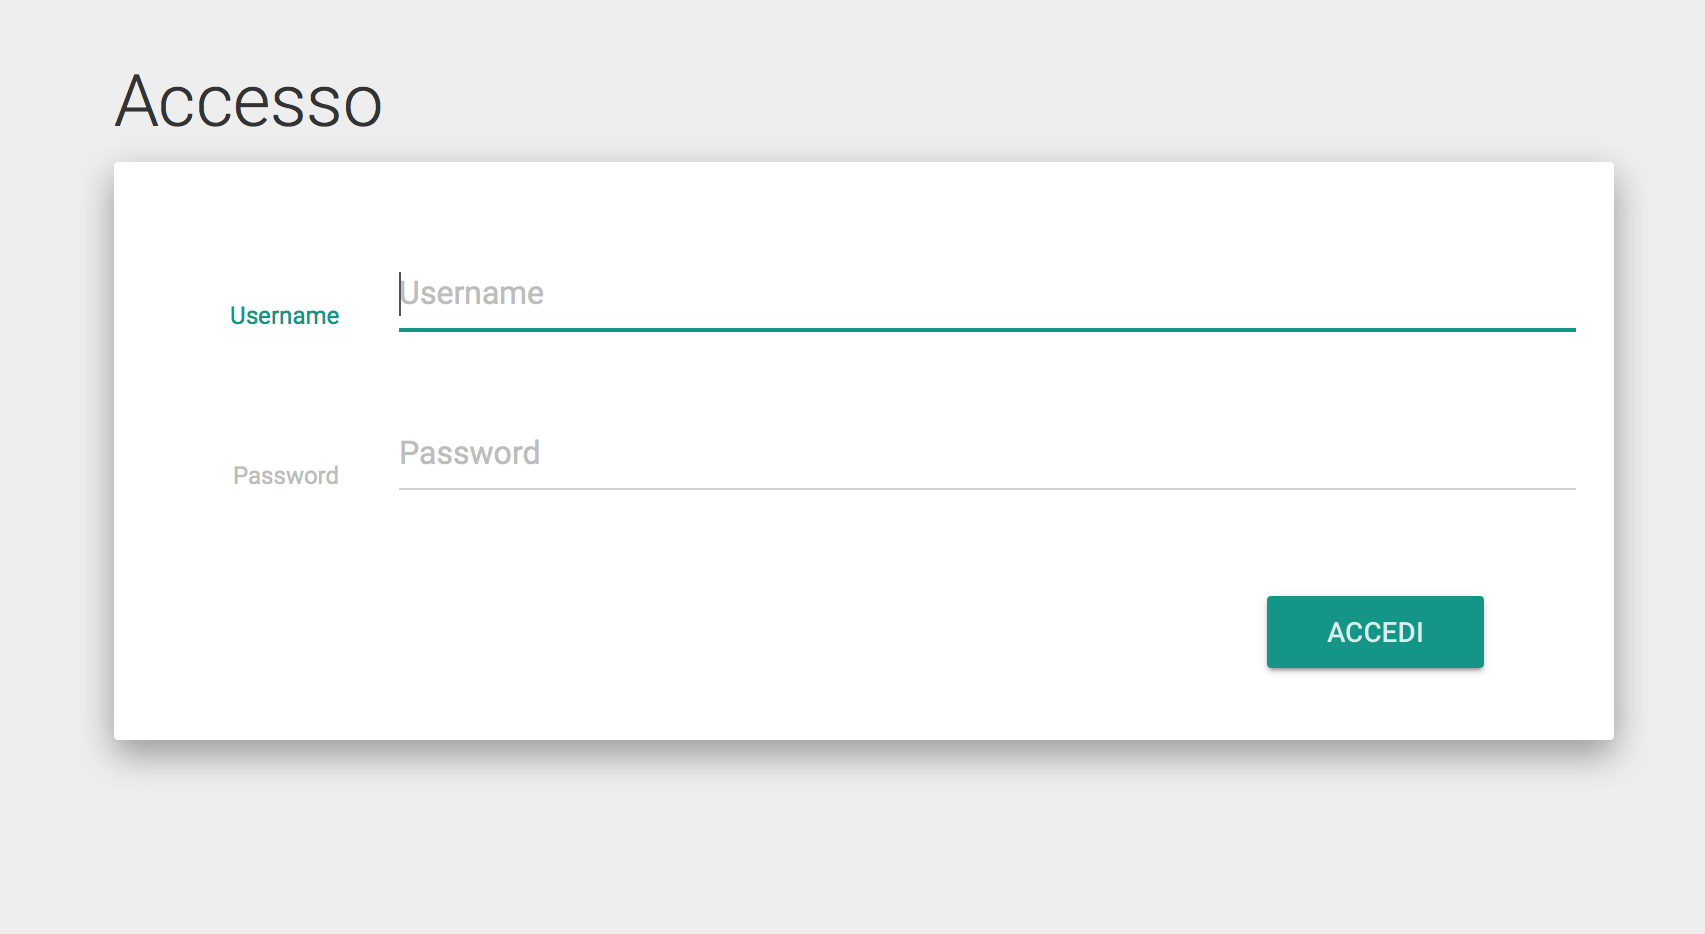
\includegraphics[width=0.8\linewidth]{../img/screenshot/loginCrop.png}
		\caption{}
		\label{Schermata di autenticazione}
		\end{figure}
		
		
	\subsection{Logout}
	Per effettuare il logout e uscire dall'applicazione è necessario aver precedentemente effettuato l'autenticazione.
	E' necessario selezionare il pulsante in alto a destra in figura.
	\begin{figure}[h]	
		\centering
		
\includegraphics[width=1.0\linewidth]{../img/screenshot/barraLogout.png}
		\caption{}
		\label{Pulsante di logout}
	\end{figure}

	\subsection{Modifica profilo personale}
	Una volta effettuato l'accesso all'applicazione, vedi \ref{autenticazione}, è possibile modificare i propri dati personali salvati nel sistema.
    
	\paragraph{Pagina di modifica profilo}
	Per accedere alla pagina delle impostazioni personali è necessario selezionare il pulsante in alto a destra sul simbolo indicato in figura.
	
	\begin{figure}[h]
		\centering
		
\includegraphics[width=1.0\linewidth]{../img/screenshot/barraImpostaz.png}
		\caption{}
		\label{Pulsante di logout}
	\end{figure}
	
	\subsubsection{Modifica username e nome completo}
	Per modificare il \mgls{username}, nome e cognome salvati è necessario:
	\begin{itemize}
		\item inserire il nome completo e/o \mgls{username};
		\item selezionare sul pulsante "SUBMIT" per confermare la modifica.
	\end{itemize}
	\begin{figure}[h]	
		\centering
		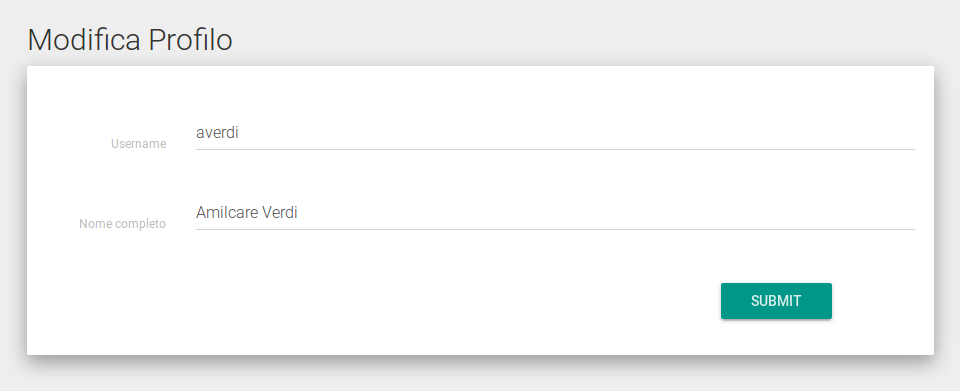
\includegraphics[width=1.0\linewidth]{../img/screenshot/user1.png}
		\caption{}
		\label{Modifica profilo}
	\end{figure}

	
	\subsection{Modifica password}
	Per modificare la password  è necessario:
	\begin{itemize}
		\item inserire la password attuale;
		\item inserire la nuova password;
		\item ripetere la nuova password;
		\item selezionare il pulsante "SUBMIT" per confermare la modifica.
	\end{itemize}
	\begin{figure}[h]
		\centering
		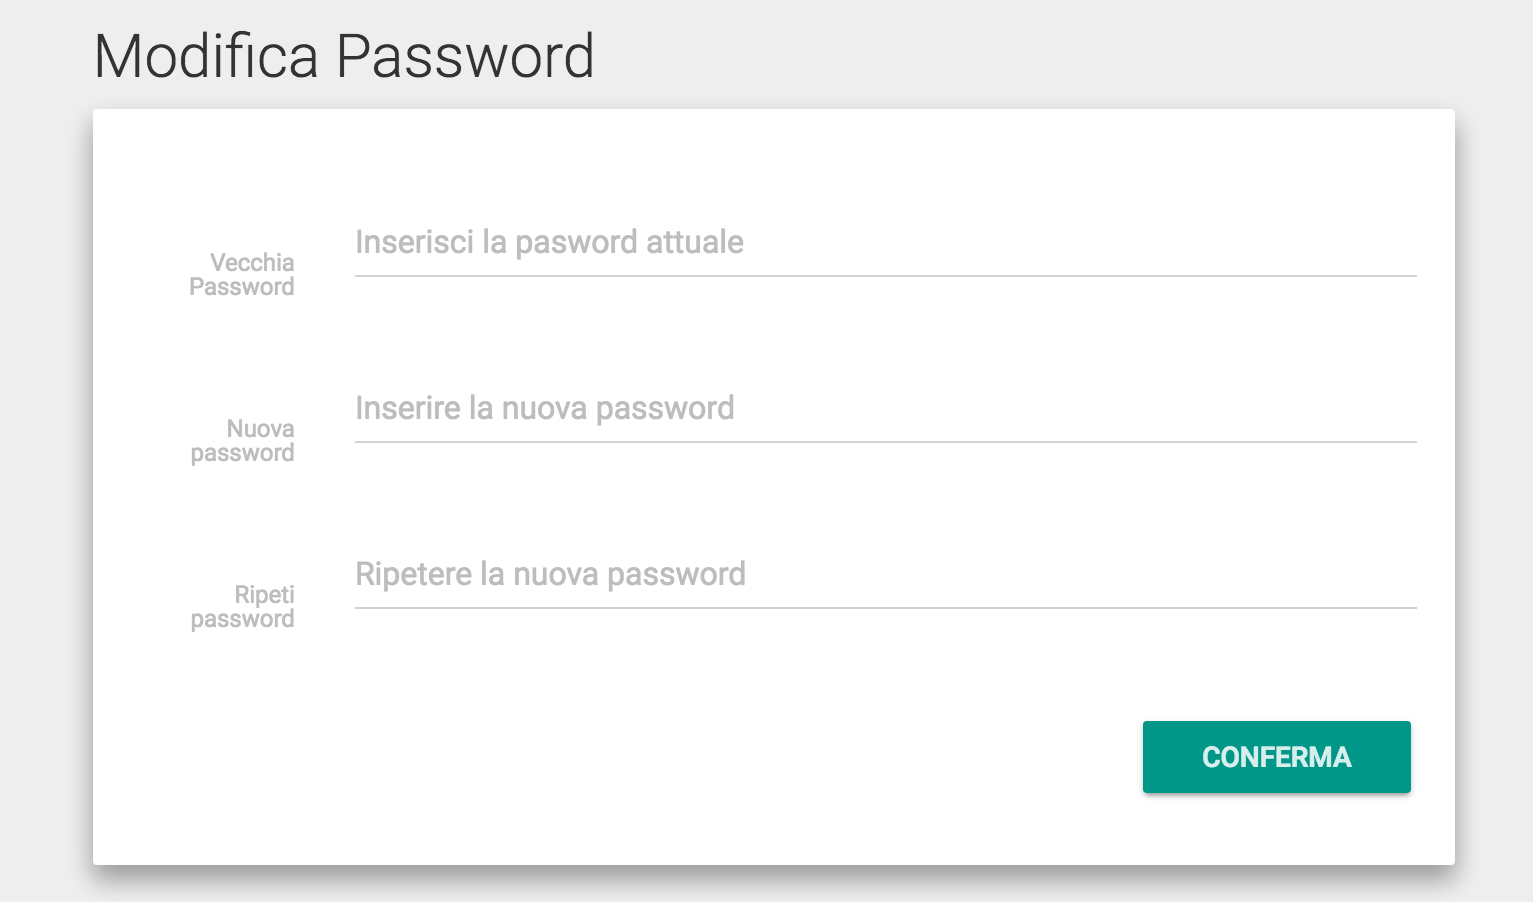
\includegraphics[width=1.0\linewidth]{../img/screenshot/user2.png}
		\caption{}
		\label{Modifica password}
	\end{figure}
	
	\newpage

	\section{Studente}\label{studente}
	Il profilo studente è il profilo  base offerto dal sistema. Ogni utente registrato dispone di tali funzionalità. Tali funzionalità sono:
	\begin{itemize}
		\item la possibilità di ricercare questionari in base a più parametri;
		\item la possibilità di esplorare i questionari presenti nel sistema per argomento;
		\item la possibilità di eseguire un questionario presente nel sistema.
	\end{itemize}
	
	\subsection{Funzionalità studente}
	\subsubsection{Ricerca questionario}\label{ricerca_questionario}
	\subsubsubsection{Pagina di ricerca  di un questionario}
	L'accesso alla pagina di ricerca questionari si effettua dal \textbf{menu laterale}. 
	E' necessario selezionare la voce "\textbf{Questionari}" nella sezione \textbf{Studente} del menu.
	\subsubsubsection{Effettuare una ricerca}
	Una volta entrati nella pagina di ricerca, è possibile inserire i parametri di ricerca nella barra apposita.
	
	\begin{figure}[H]	
		\centering
		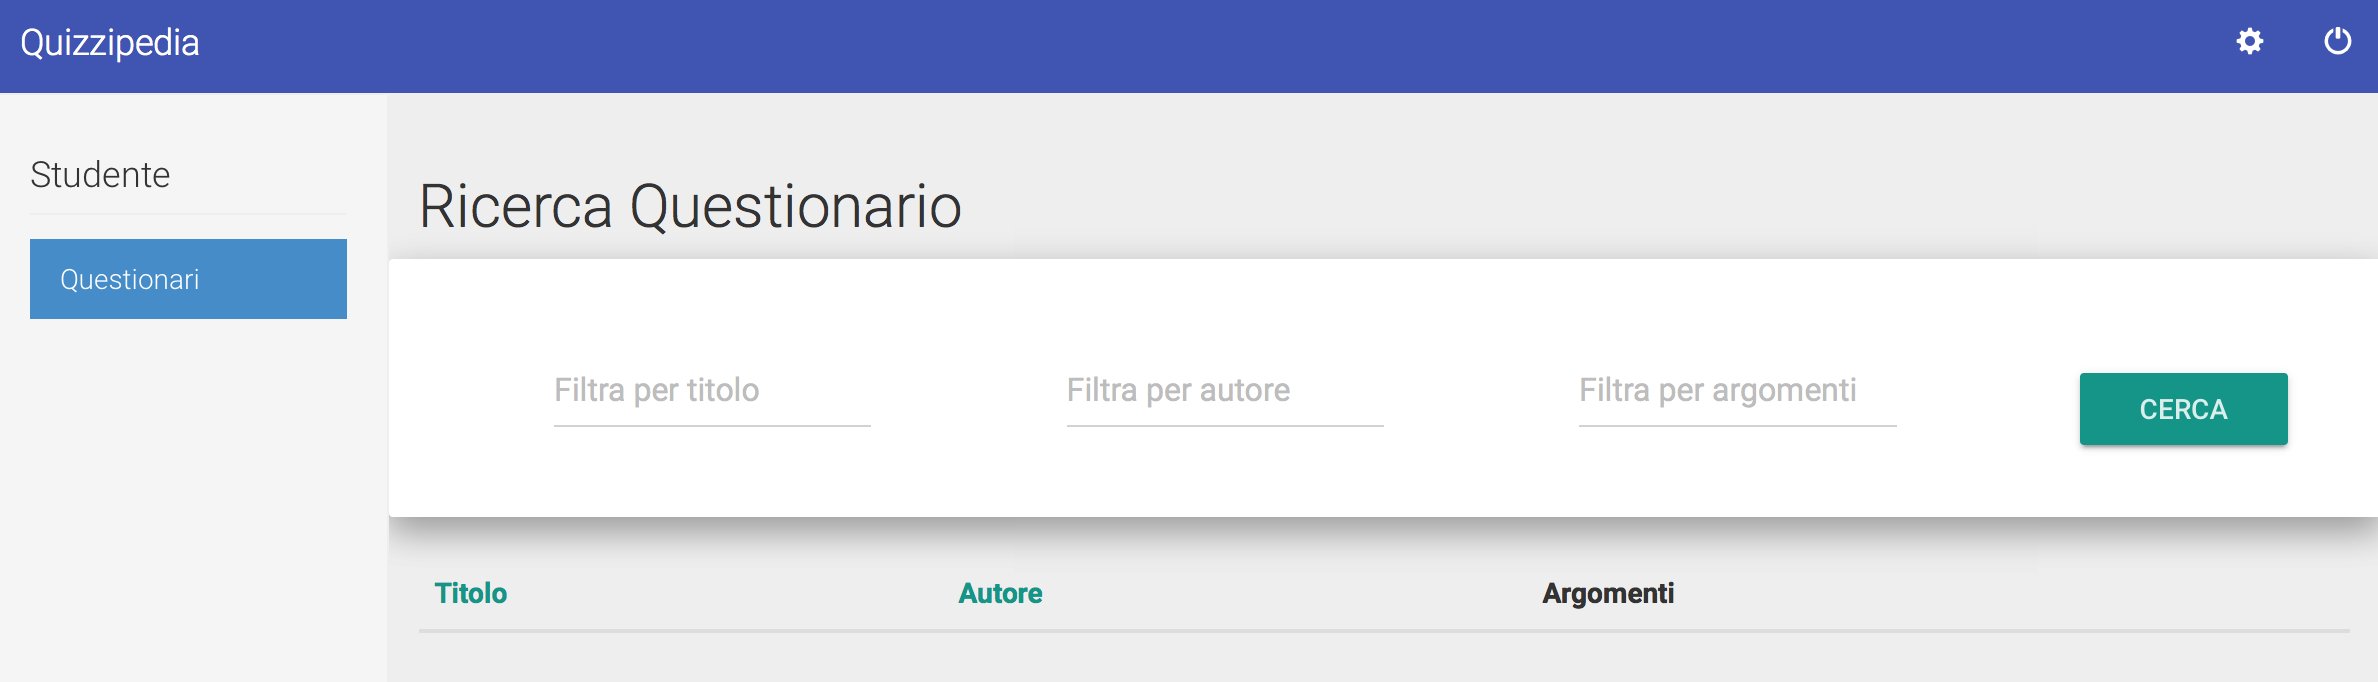
\includegraphics[width=1.0\linewidth]{../img/screenshot/ricercaQuestionario.png}
		\caption{}
		\label{Ricerca questionario}
	\end{figure}
	
	E' possibile inserire dei filtri per la ricerca. 
	
	\begin{figure}[H]		
		\centering
		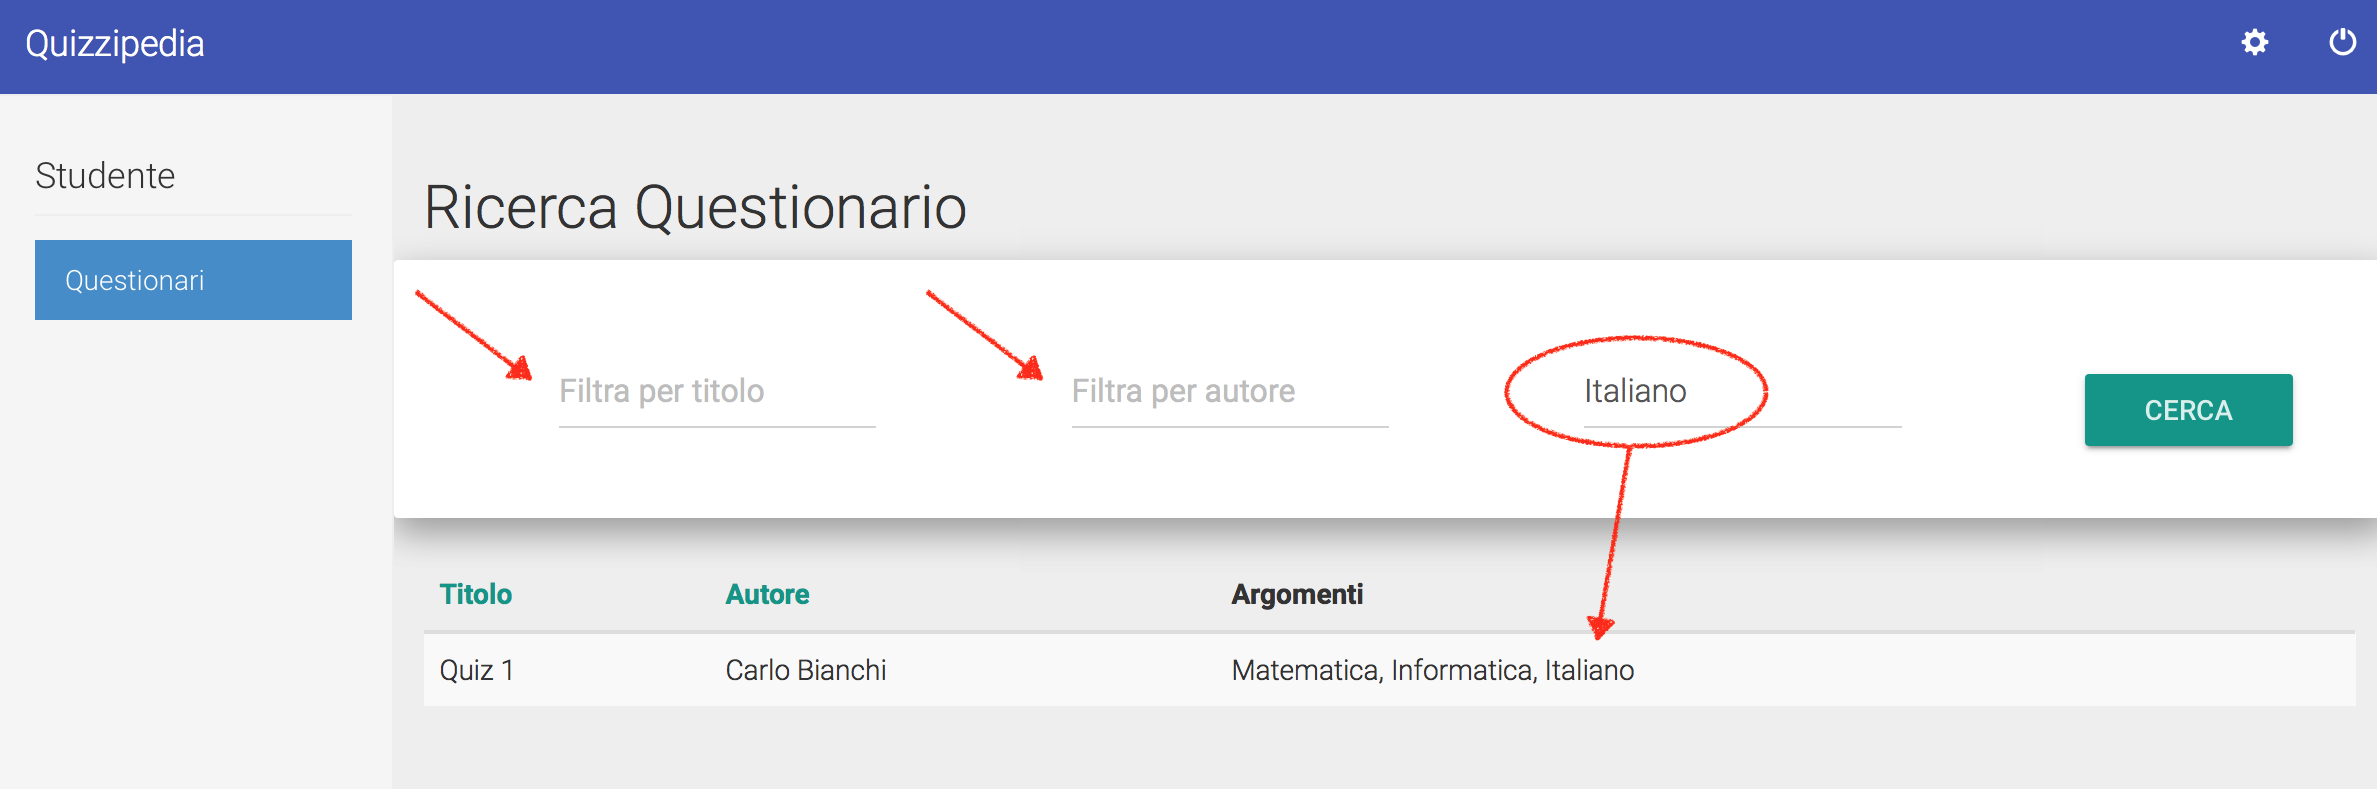
\includegraphics[width=1.0\linewidth]{../img/screenshot/filtriRicerca.png}
		\caption{}
		\label{Ricerca questionario con filtri}
	\end{figure}
	
	
	\subsubsection{Esplorazione argomenti}	
	
	\subsubsubsection{Pagina di esplorazione argomenti} \label{esplorazione_arg}
	L'accesso alla pagina di esplorazione degli argomenti e si effettua dal \textbf{menu laterale}. 
	E' necessario selezionare la voce "\textbf{Esplora argomenti}" nella sezione \textbf{Studente} del menu.
	\subsubsubsection{Navigare tra gli argomenti}
	Dalla pagina di esplorazione degli argomenti è possibile vedere quali argomenti sono disponibili nel sistema. Cliccando su un argomento è possibile vedere i sottoargomenti e i relativi questionari disponibili.
	
	\subsubsection{Esecuzione questionario}
	\subsubsubsection{Trovare il questionario}
	Per trovare un questionario da eseguire è possibile effettuare una ricerca, vedi \ref{ricerca_questionario}.
	Oppure è possibile sceglierlo in base all'argomento, vedi \ref{esplorazione_arg}.
	\subsubsection{Eseguire un questionario}
	Una  volta trovato il questionario desiderato, è possibile eseguirlo cliccando sul tasto "esegui" a fianco ad esso.
	Durante l'esecuzione di un questionario sarà possibile navigare tra le domande presenti con i tasti "precedente" e Wsuccessiva".
	Una volta terminato di segnare le risposte, cliccando sul tasto "conferma" sarà possibile vedere la soluzione del questionario svolto.
	Attenzione, tutte le domande devono essere compilate affinché sia possibile visualizzarne la correzione.
	Per abbandonare il questionario in esecuzione basterà premere "abbandona", e si verrà riportati alla schermata precedente all'inizio dell'esecuzione.
	
	\begin{figure}[H]	
		\centering
		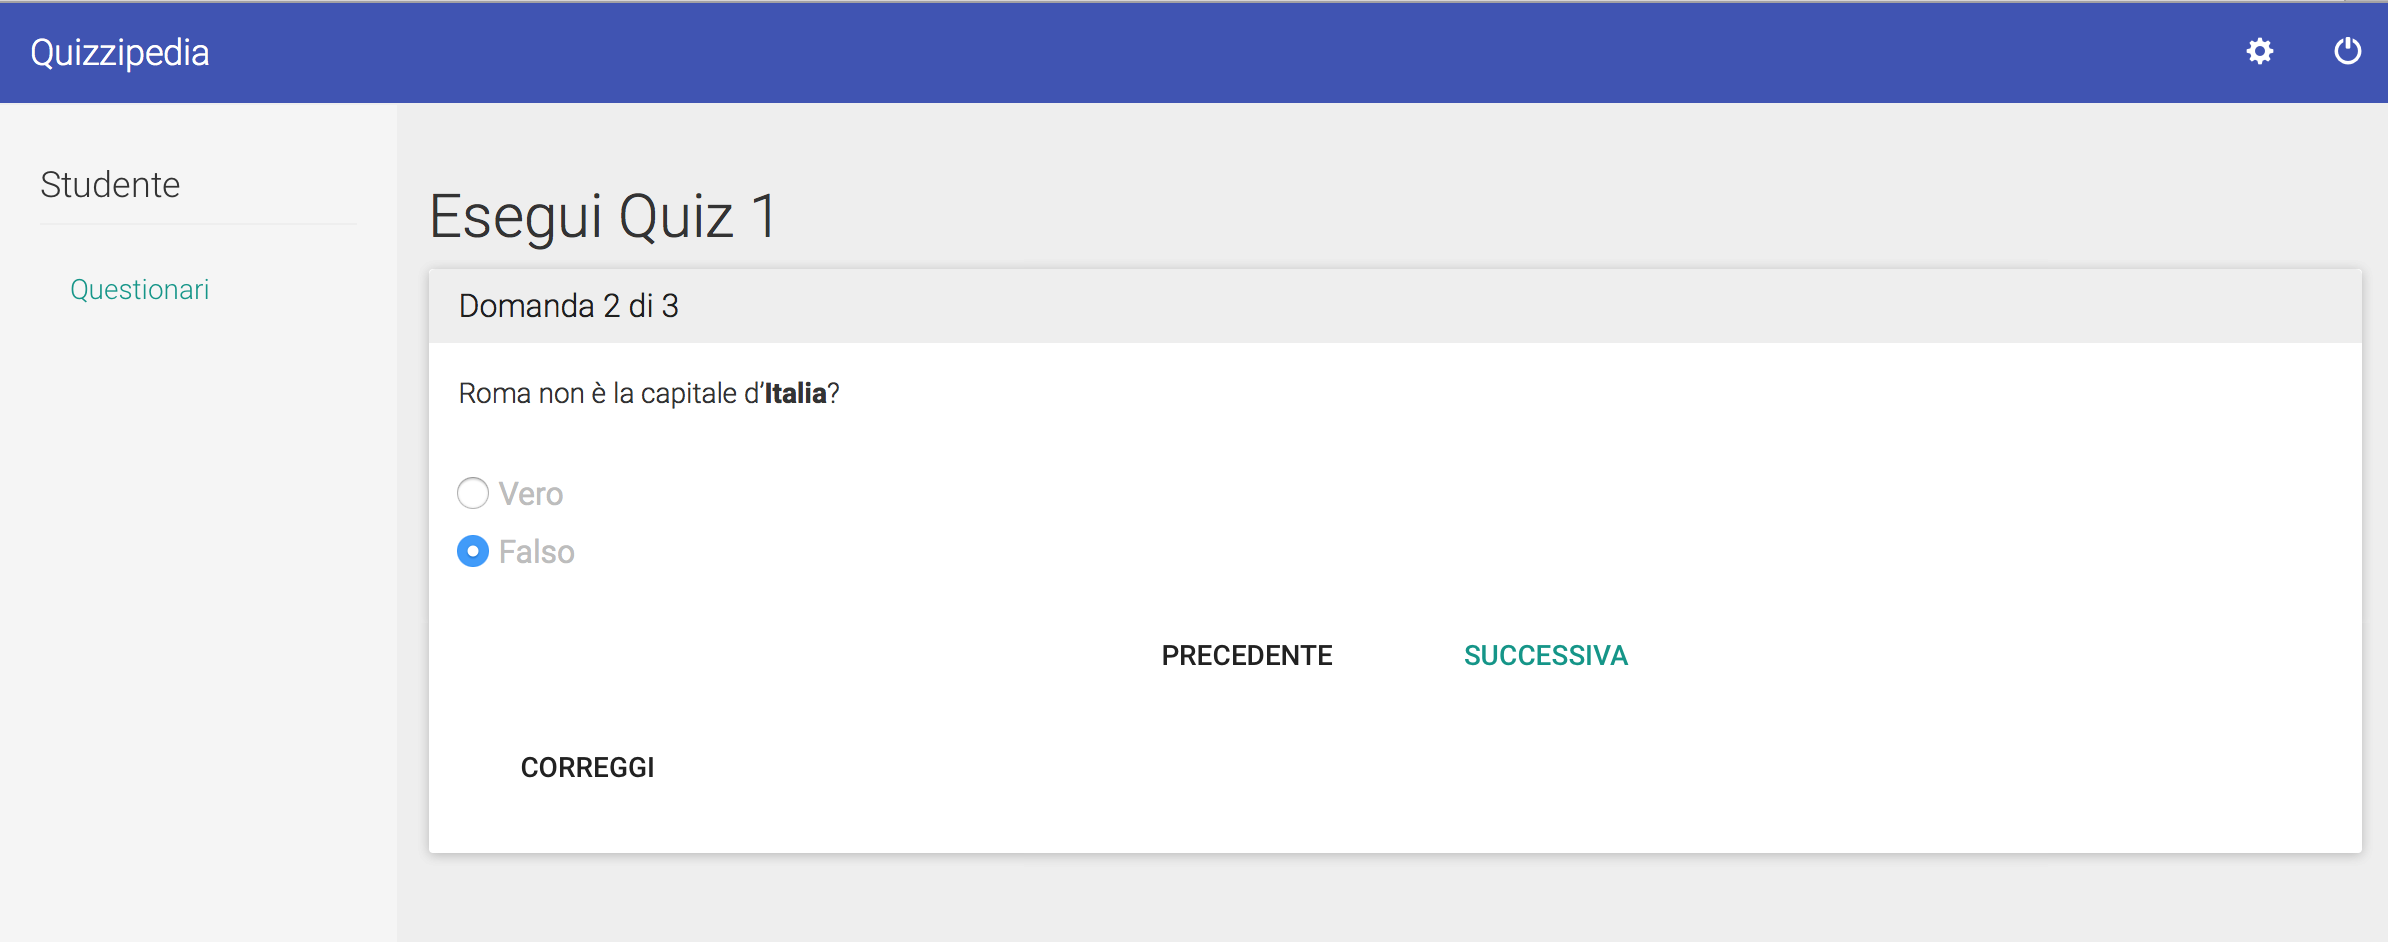
\includegraphics[width=1.0\linewidth]{../img/screenshot/esecuzioneQuestionario.png}
		\caption{}
		\label{Eseguire questionario}
	\end{figure}
	
	\section{Docente}\label{docente}
	Un profilo docente ha accesso a tutte le funzionalità di uno studente.Per informazioni dettagliate su tali funzionalità si veda la sezione \ref{studente}
		Inoltre offre funzionalità aggiuntive quali:
		\begin{itemize}
			\item la possibilità di gestire questionari (aggiungerli, rimuoverli e modificarli);
			\item la possibilità di gestire domande (aggiungerle, rimuoverle e modificarle);
			\item la possibilità di gestire argomenti (aggiungerli, rimuoverli e modificarli)
		\end{itemize}
	\subsection{Funzionalità docente}
	
    \subsubsection{Gestione domande}

    Selezionando la voce "domande" dal menu a lato, sotto la voce "Docente", vengono visualizzate le domande precedentemente create. 
	\subsubsubsection{Creazione domanda}
	Per creare una nuova domanda è sufficiente premere il taso in alto a destra nella pagina "gestione domande". 
	Si aprirà un form apposito per l'inserimento del \mgls{qml} per la descrizione della domanda.
	Una volta inserito il \mgls{qml}, selezionare il pulsante "crea" in basso a destra.
	
	\paragraph{Attenzione !!}Se il \mgls{qml} inserito non è valido, l'applicazione chiederà di correggere il \mgls{qml} inserito e di selezionare nuovamente il pulsante "crea".
	\subsubsubsection{Modifica domanda}
	Per modificare una domanda è necessario selezionare la domanda che si desidera modificare. Si aprirà una schermata che permetterà di editare il \mgls{qml} della domanda scelta.
	Una volta modificata la domanda, premere il pulsante "submit" in basso a destra per confermare le modifiche effettuate. Con il pulsante "calcel" si evita di effettuare in modo permanente le modifiche appena fatte.
	Se il \mgls{qml} modificato non risulta corretto, il sistema chiederà di correggere il \mgls{qml} inserito prima di salvare nuovamente.
	
		\begin{figure}[H]	
			\centering
			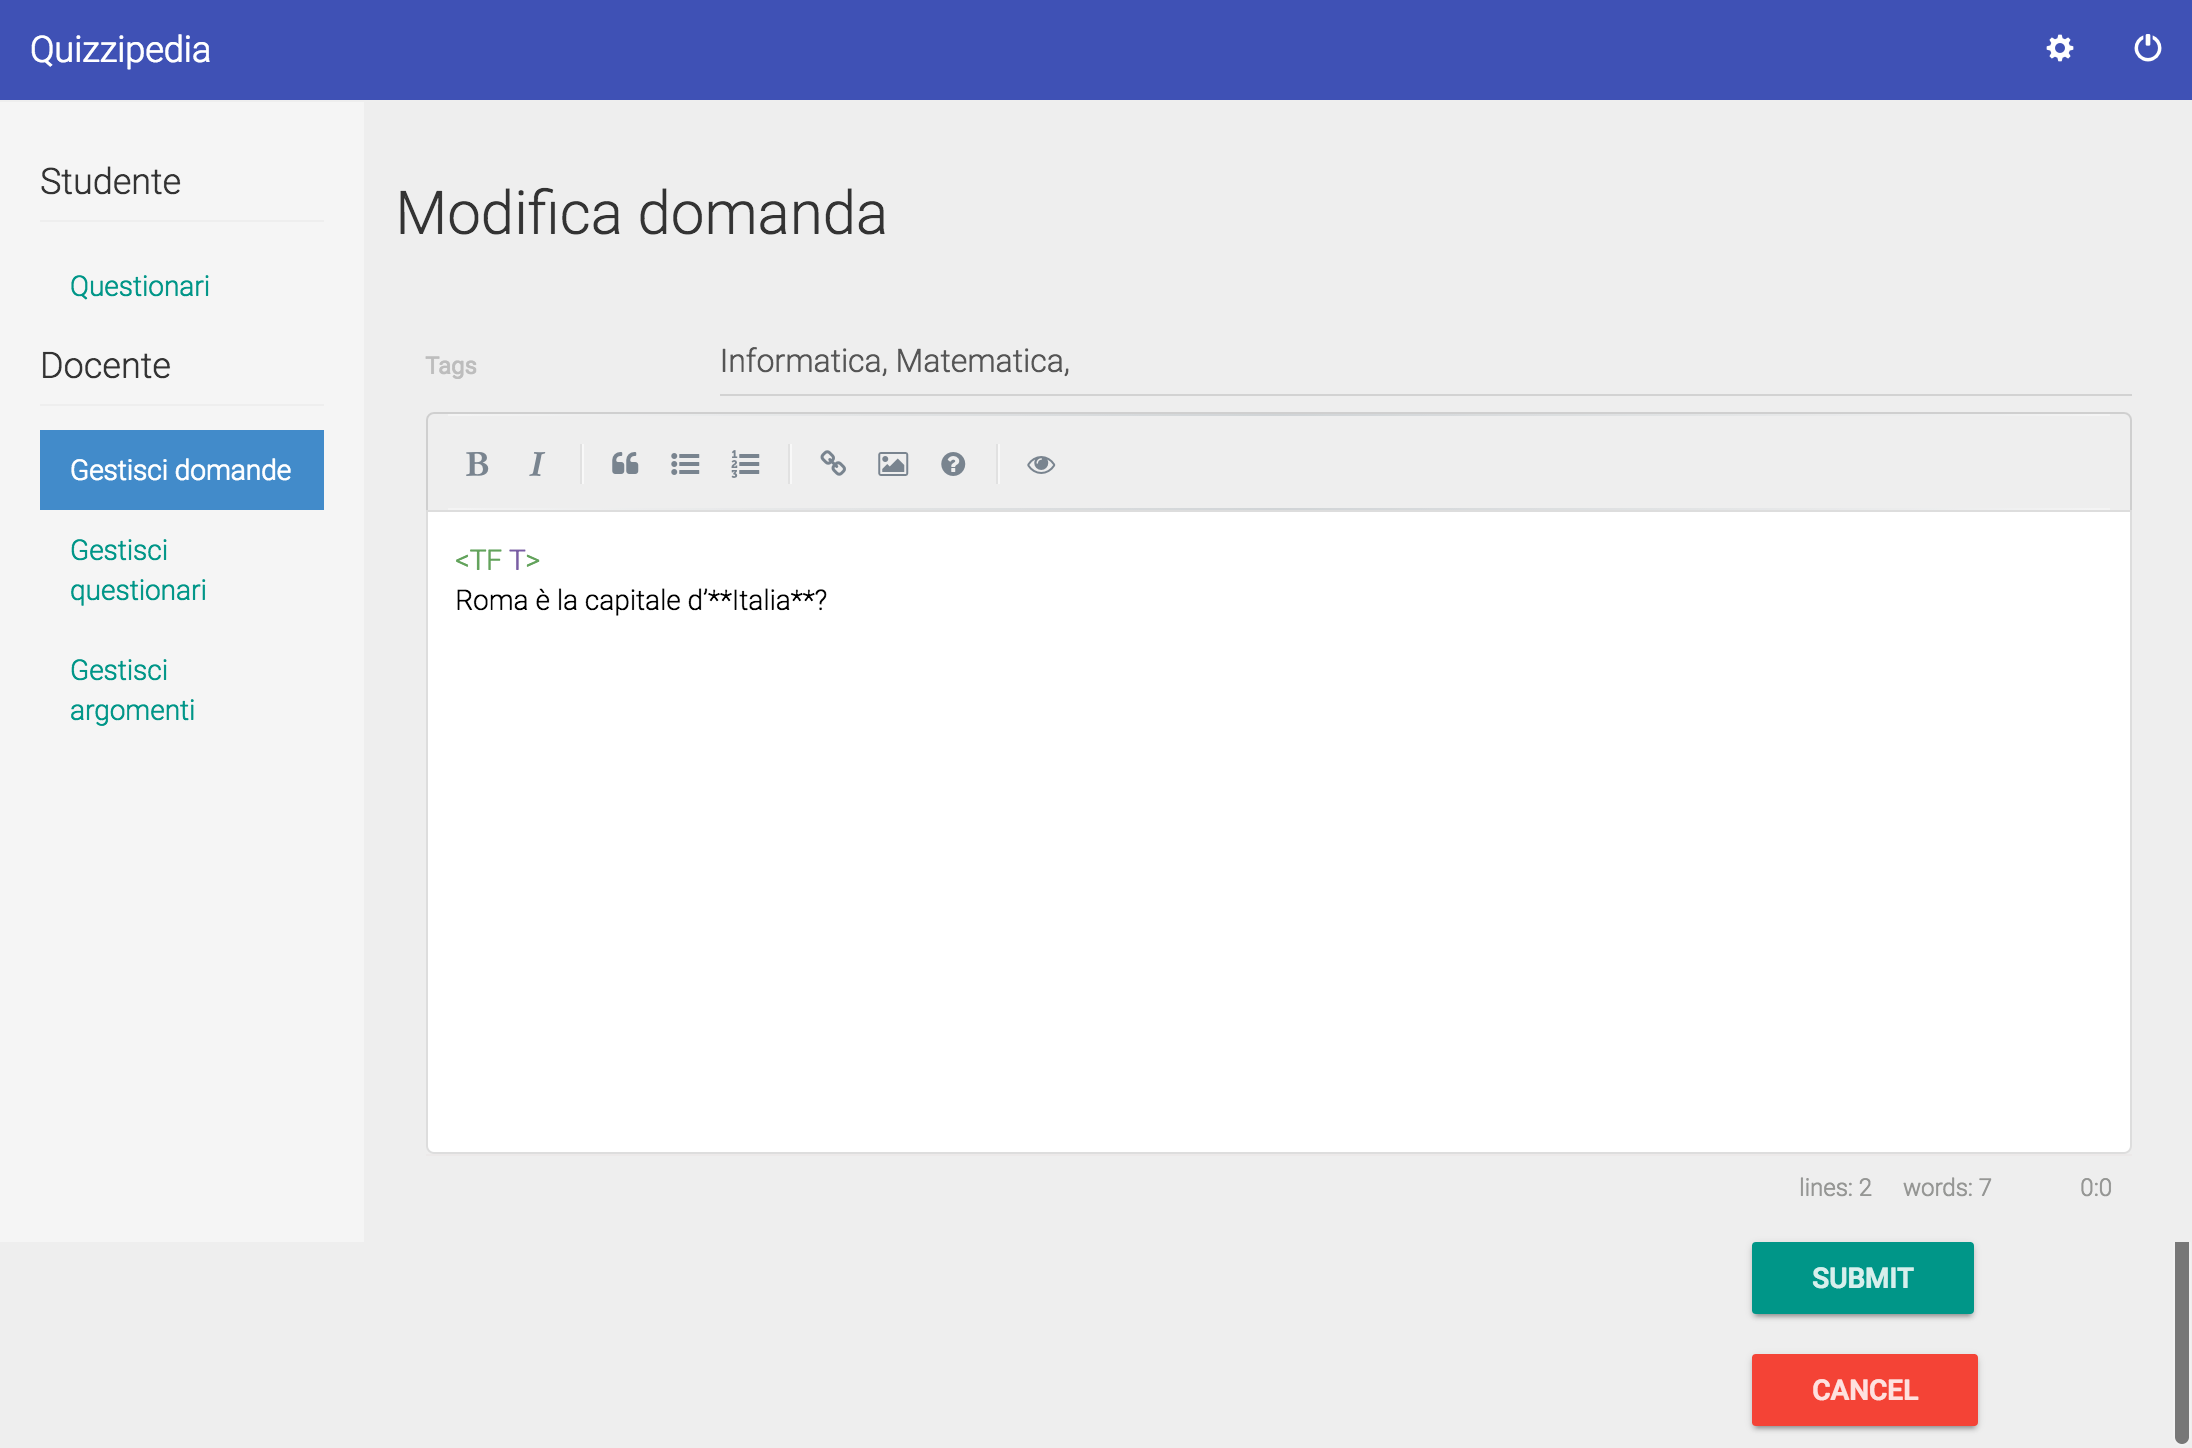
\includegraphics[width=0.5\linewidth]{../img/screenshot/modificaDomanda.png}
			\caption{}
			\label{Modifica domanda}
		\end{figure}
	
	\subsubsubsection{Eliminazione domanda}
	Per eliminare una domanda è necessario selezionare la voce "elimina" a fianco della domanda da eliminare. Prima di eliminare la domanda definitivamente il sistema chiederà di confermare nuovamente l'eliminazione.
	Verrà aperta una finestra che chiederà di confermare o annullare l'eliminazione. Cliccando la voce "elimina", la domanda selezionata verrà eliminata irreversibilmente. Cliccando la voce "annulla", il procedimento di eliminazione verrà interrotto e la domanda non verrà eliminata.
	
	\begin{figure}[H]	
		\centering
		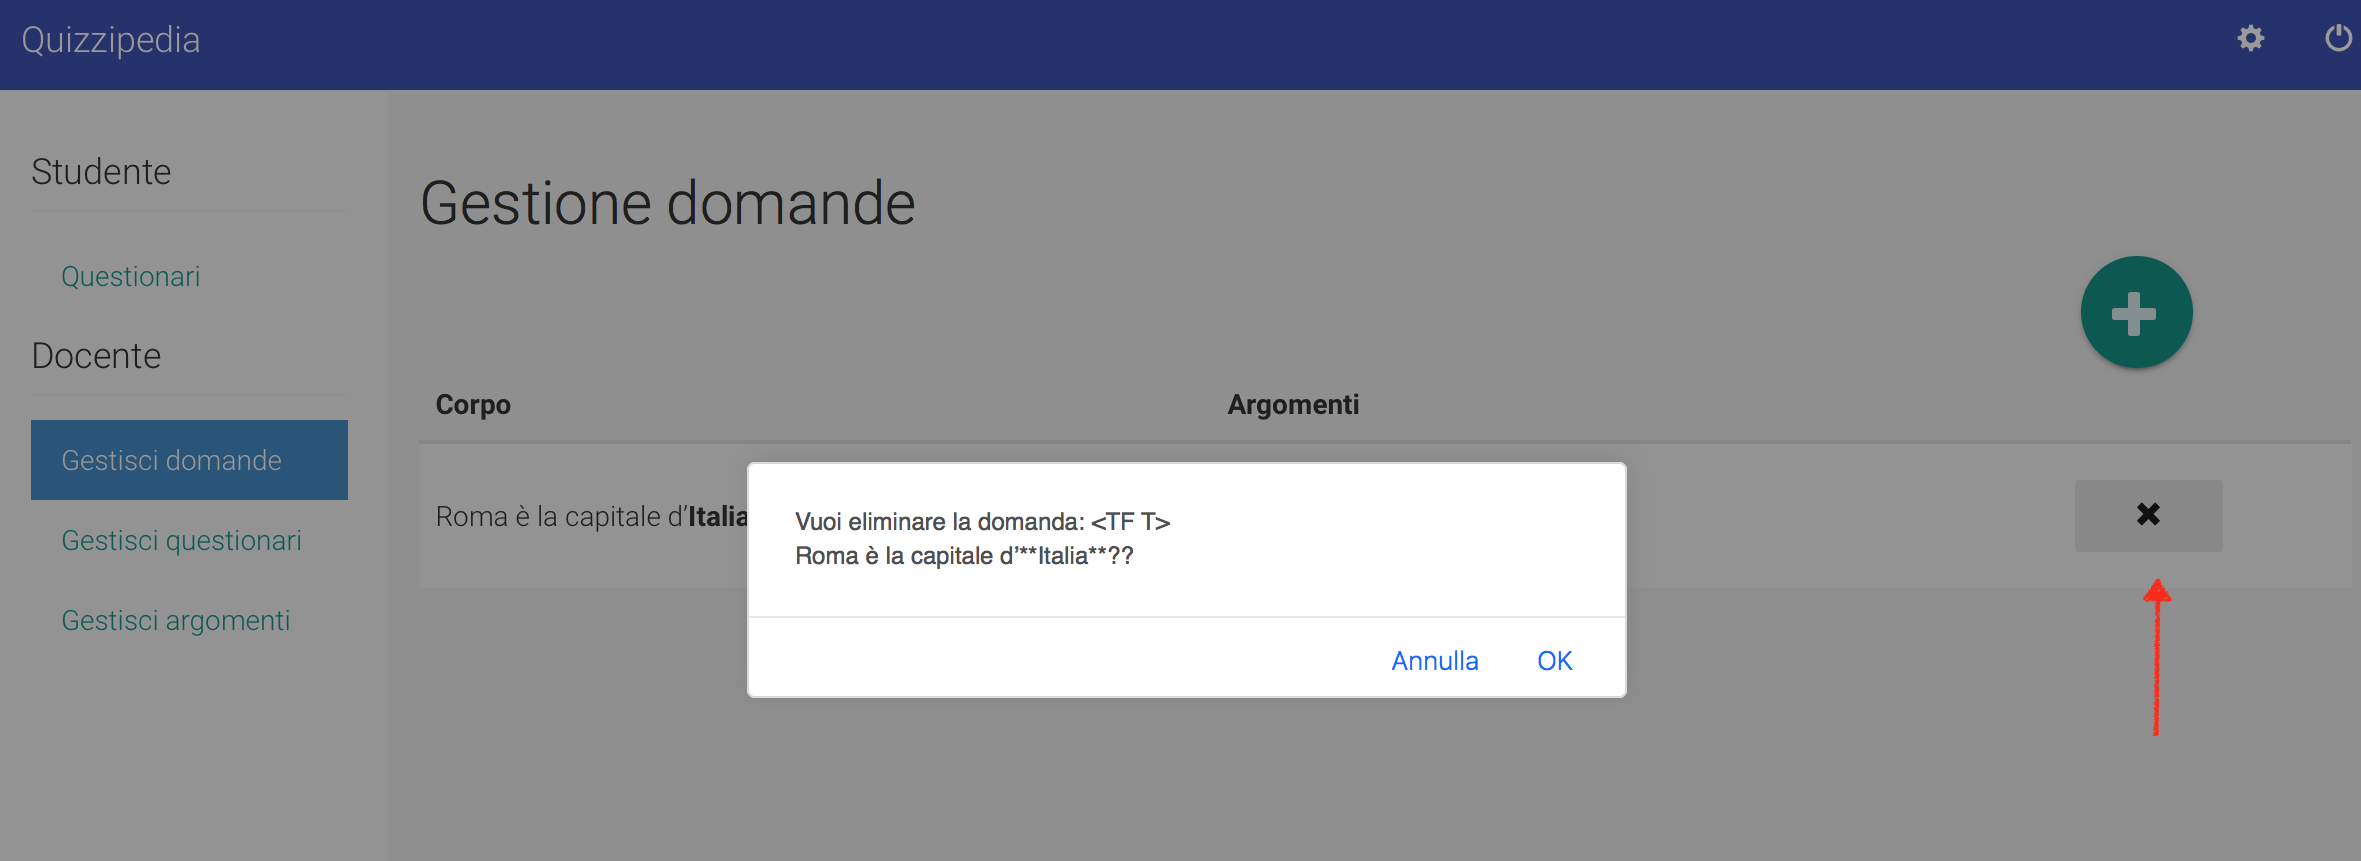
\includegraphics[width=1.0\linewidth]{../img/screenshot/eliminaDomanda.png}
		\caption{}
		\label{Elimina domanda}
	\end{figure}
		
	\subsubsection{Gestione argomenti}
	Selezionando la voce "argomenti" dal menu a lato, sotto la voce "Docente", vengono visualizzati gli argomenti precedentemente creati.
		\subsubsubsection{Creazione argomenti}
		Per creare un nuovo argomento è necessario editare il nome del nuovo argomento e la sua descrizione ed infine selezionare il simbolo "+" in alto a destra, nella pagina "argomenti" del menu "Docente".
		
		Sarà necessario 
			\begin{itemize}
			\item il nome del argomento;
			\item la descrizione dell'argomento;
			\item selezionare "crea" per confermare la creazione del argomento.
		\end{itemize}
		
			\begin{figure}[H]	
				\centering
				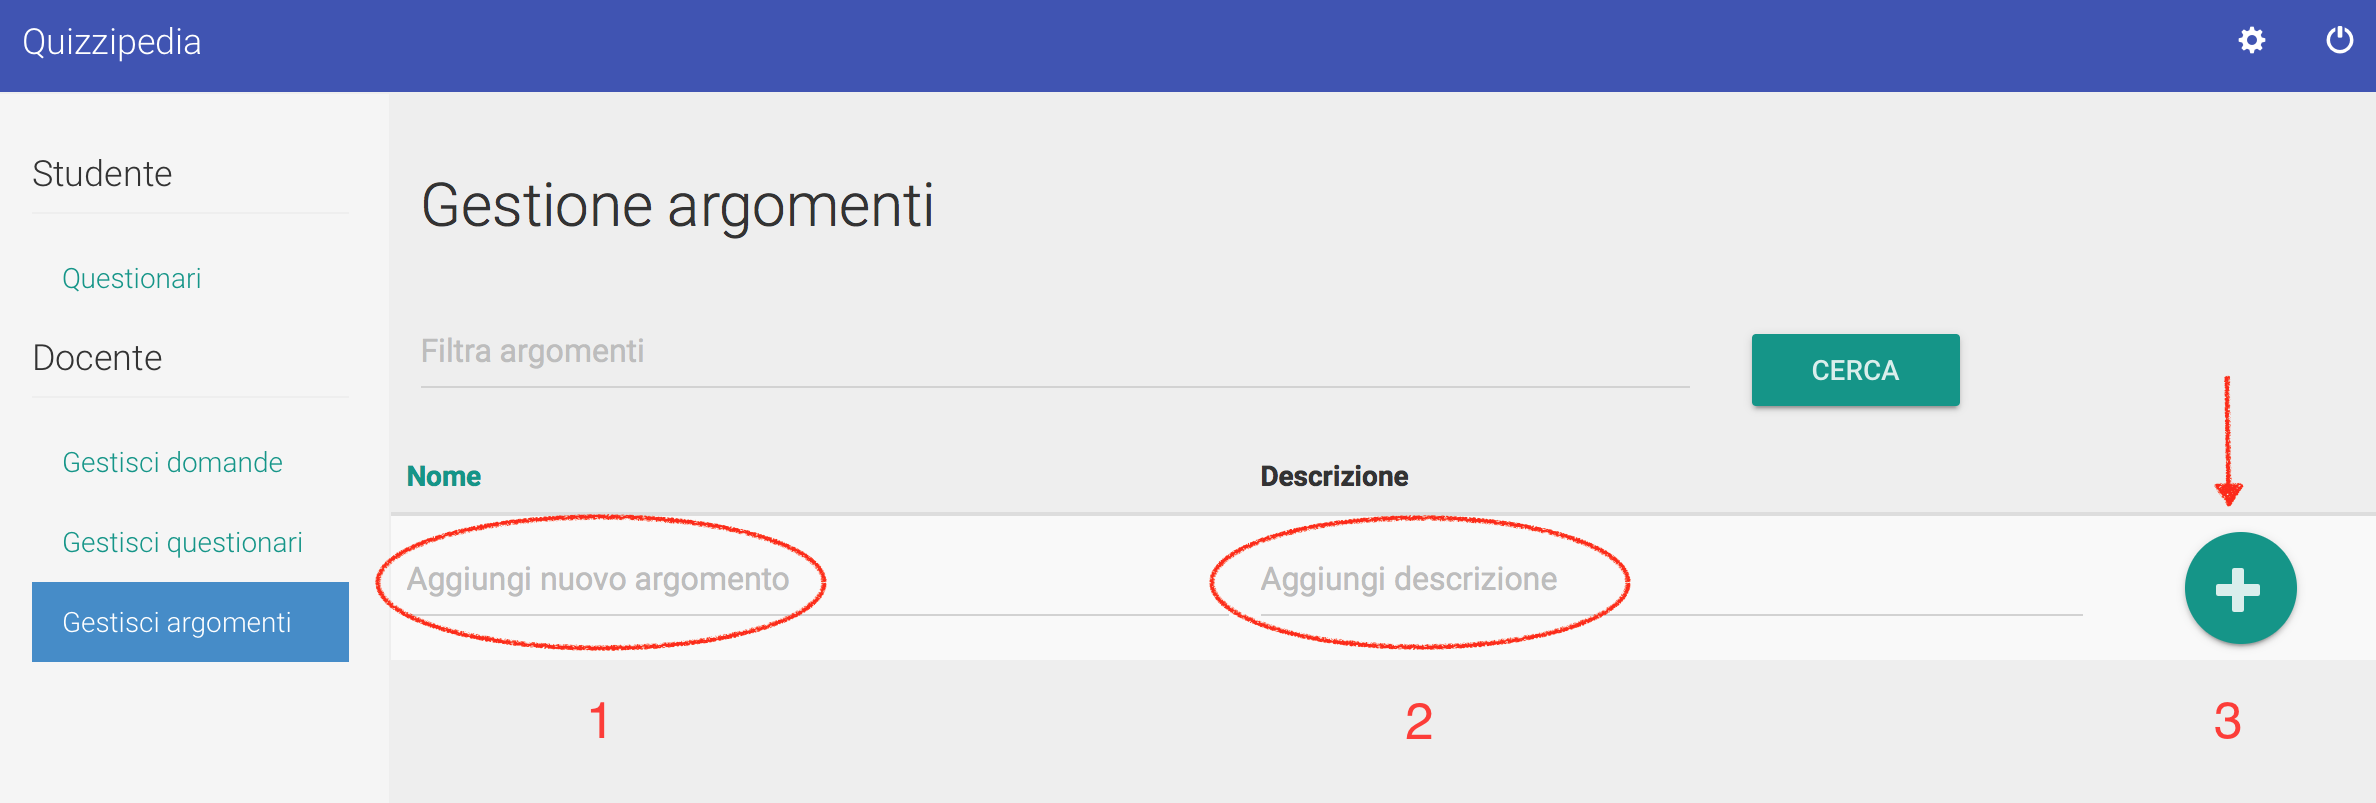
\includegraphics[width=1.0\linewidth]{../img/screenshot/aggiungiArgomento.png}
				\caption{}
				\label{Creazione argomento}
			\end{figure}
		
		Una volta creato un nuovo argomento, questo comparirà nella schermata degli argomenti precedentemente creati.
		
		\subsubsubsection{Modifica argomento}
		Per modificare un argomento è necessario editare sul nome o sulla descrizione  dell'argomento che di vuole modificare. In questo momento il pulsante con la spunta sarà abilitato alla pressione. Si presenterà ora in color verde e la madifica effettiva dell'argomento sarà effettuata solo alla pressione di questo pulsante che tornerà poi disabilitato.
		
			\begin{figure}[H]	
				\centering
				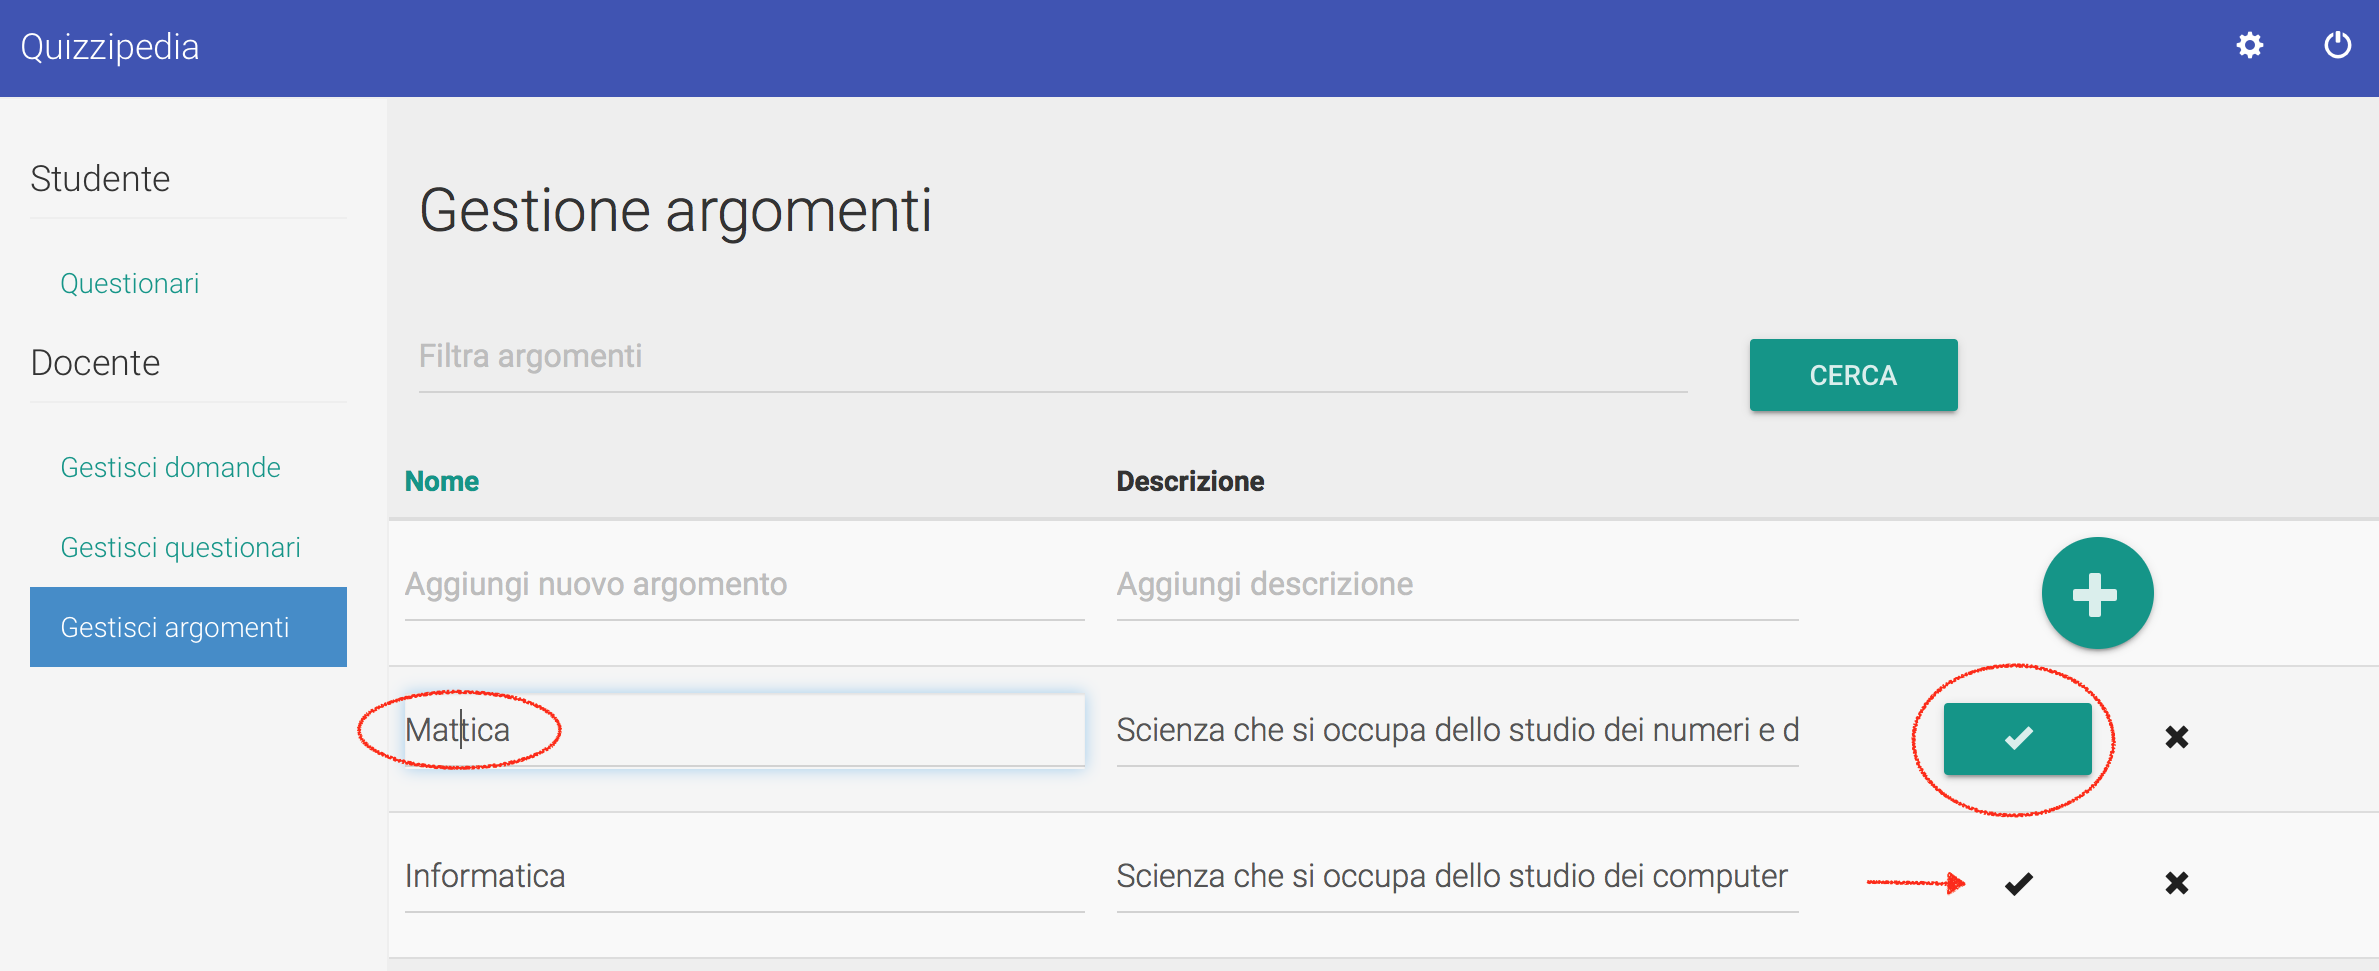
\includegraphics[width=1.0\linewidth]{../img/screenshot/modificaArgomento.png}
				\caption{}
				\label{Modifica argomento}
			\end{figure}
		
		\subsubsubsection{Eliminazione argomento}
		Per eliminare un argomento è necessario selezionare la voce "x" a fianco del argomento da eliminare. Prima di eliminare un argomento definitivamente, il sistema chiederà di confermare nuovamente l'eliminazione.
		Verrà aperta una finestra che chiederà di confermare o annullare l'eliminazione. Cliccando la voce "elimina", l'argomento selezionato verrà eliminato irreversibilmente. Cliccando la voce "annulla", il procedimento di eliminazione verà interrotto e il argomento non verrà eliminato.
		Non possono essere eliminati gli argomenti che hanno domande o questionari associati.
		
			\begin{figure}[H]	
				\centering
				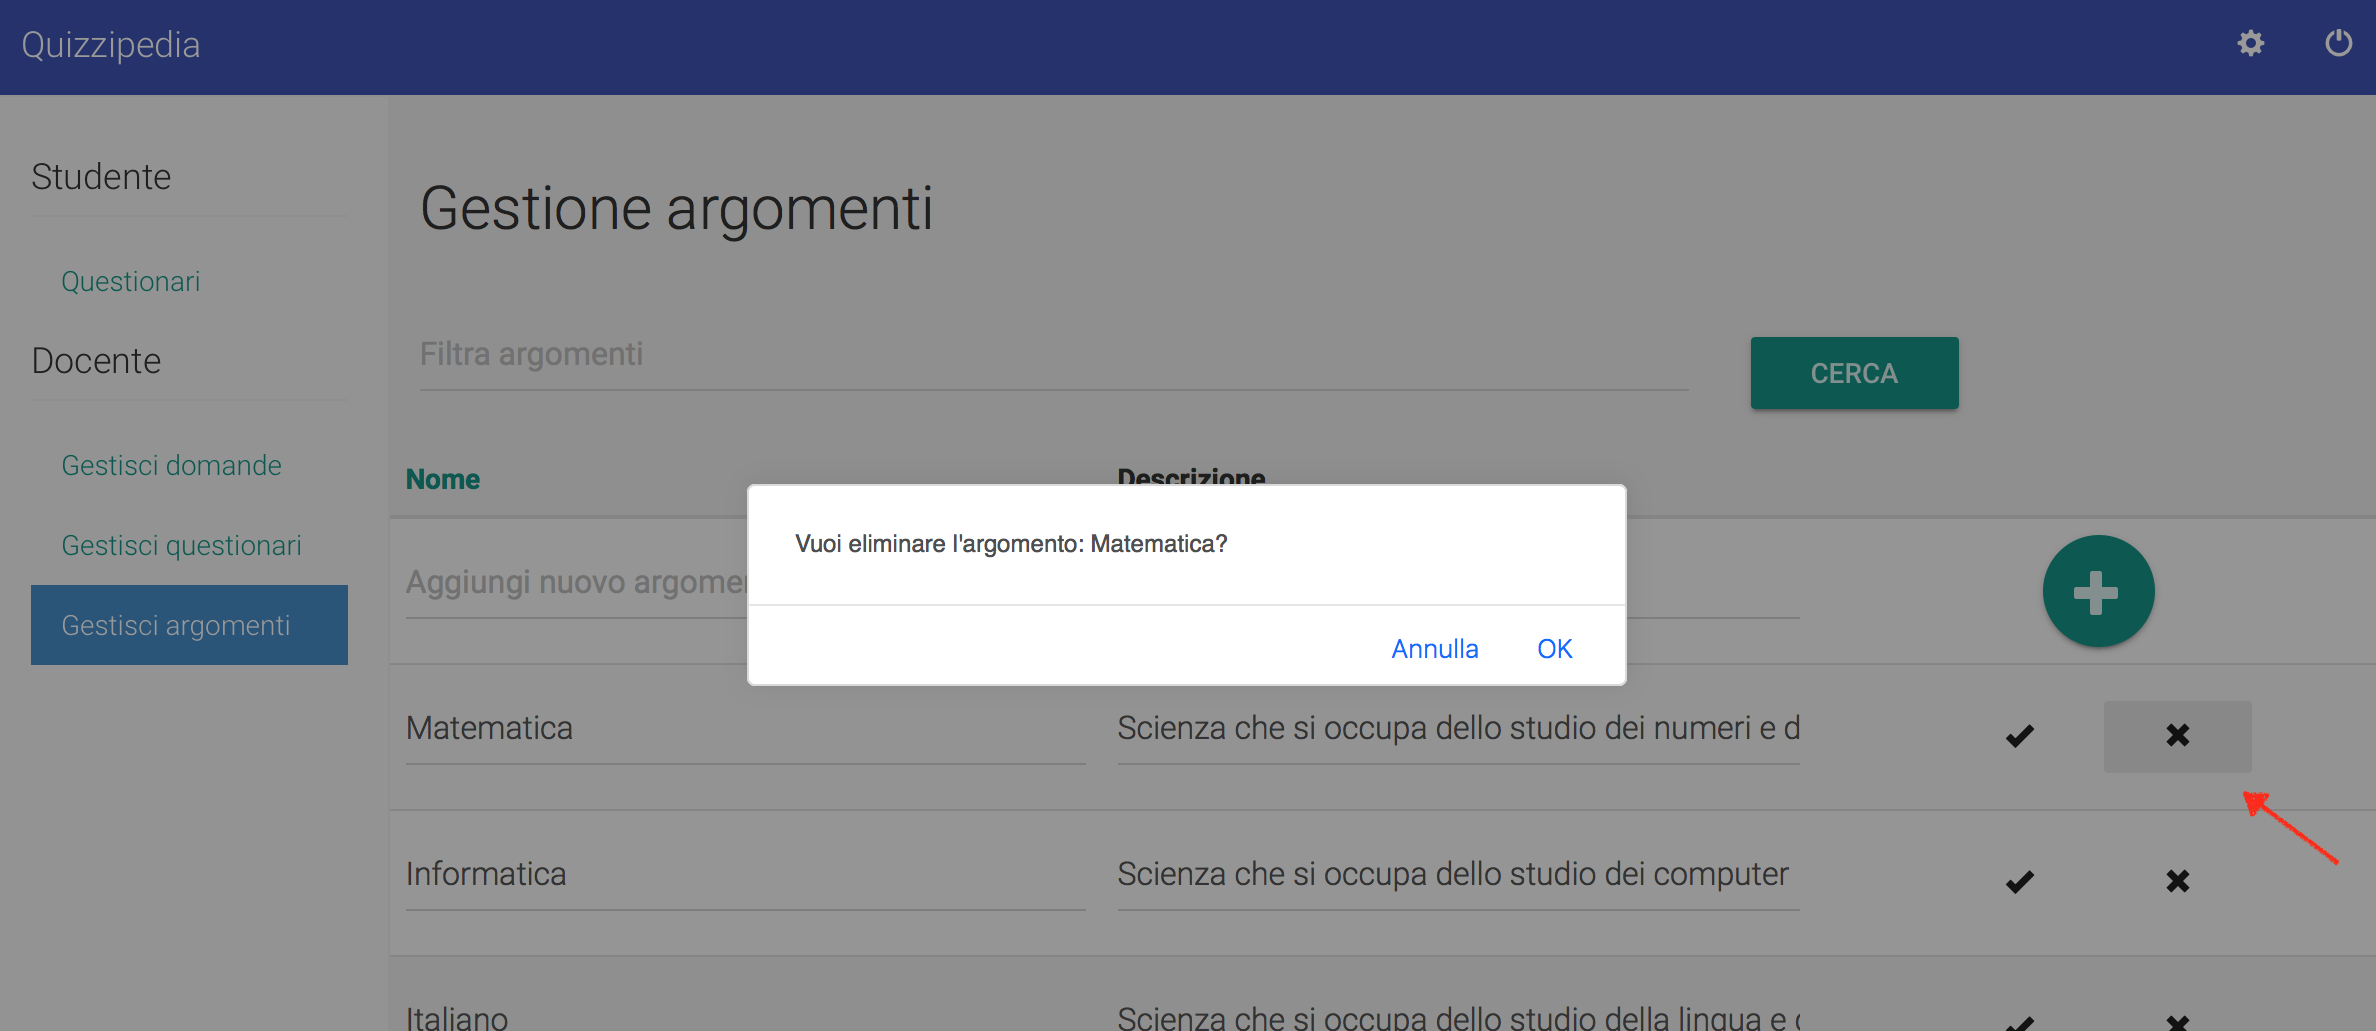
\includegraphics[width=1.0\linewidth]{../img/screenshot/eliminaArgomento.png}
				\caption{}
				\label{Elimina argomento}
			\end{figure}
		
		\subsubsection{Gestione questionario}
		\subsubsubsection{Creazione questionario}
		Per creare un questionario è necessario selezionare "+" in alto a destra della pagina. Si aprirà una schermata che permetterà di inserire il titolo del questionario, di aggiungere le domande e di aggiungere gli argomenti al questionario corrente.
		Una volta terminata la modifica, selezionare la voce "submit" per creare il nuovo questionario costruito. 
		Per annullare l'operazione di creazione del questionario selezionare "cancel".
		
		Nel caso il questionario creato non rispetti le regole per la definizione di un questionario, il sistema chiederà di modificare il questionario prima di salvare nuovamente.
		
		\begin{figure}[H]	
			\centering
			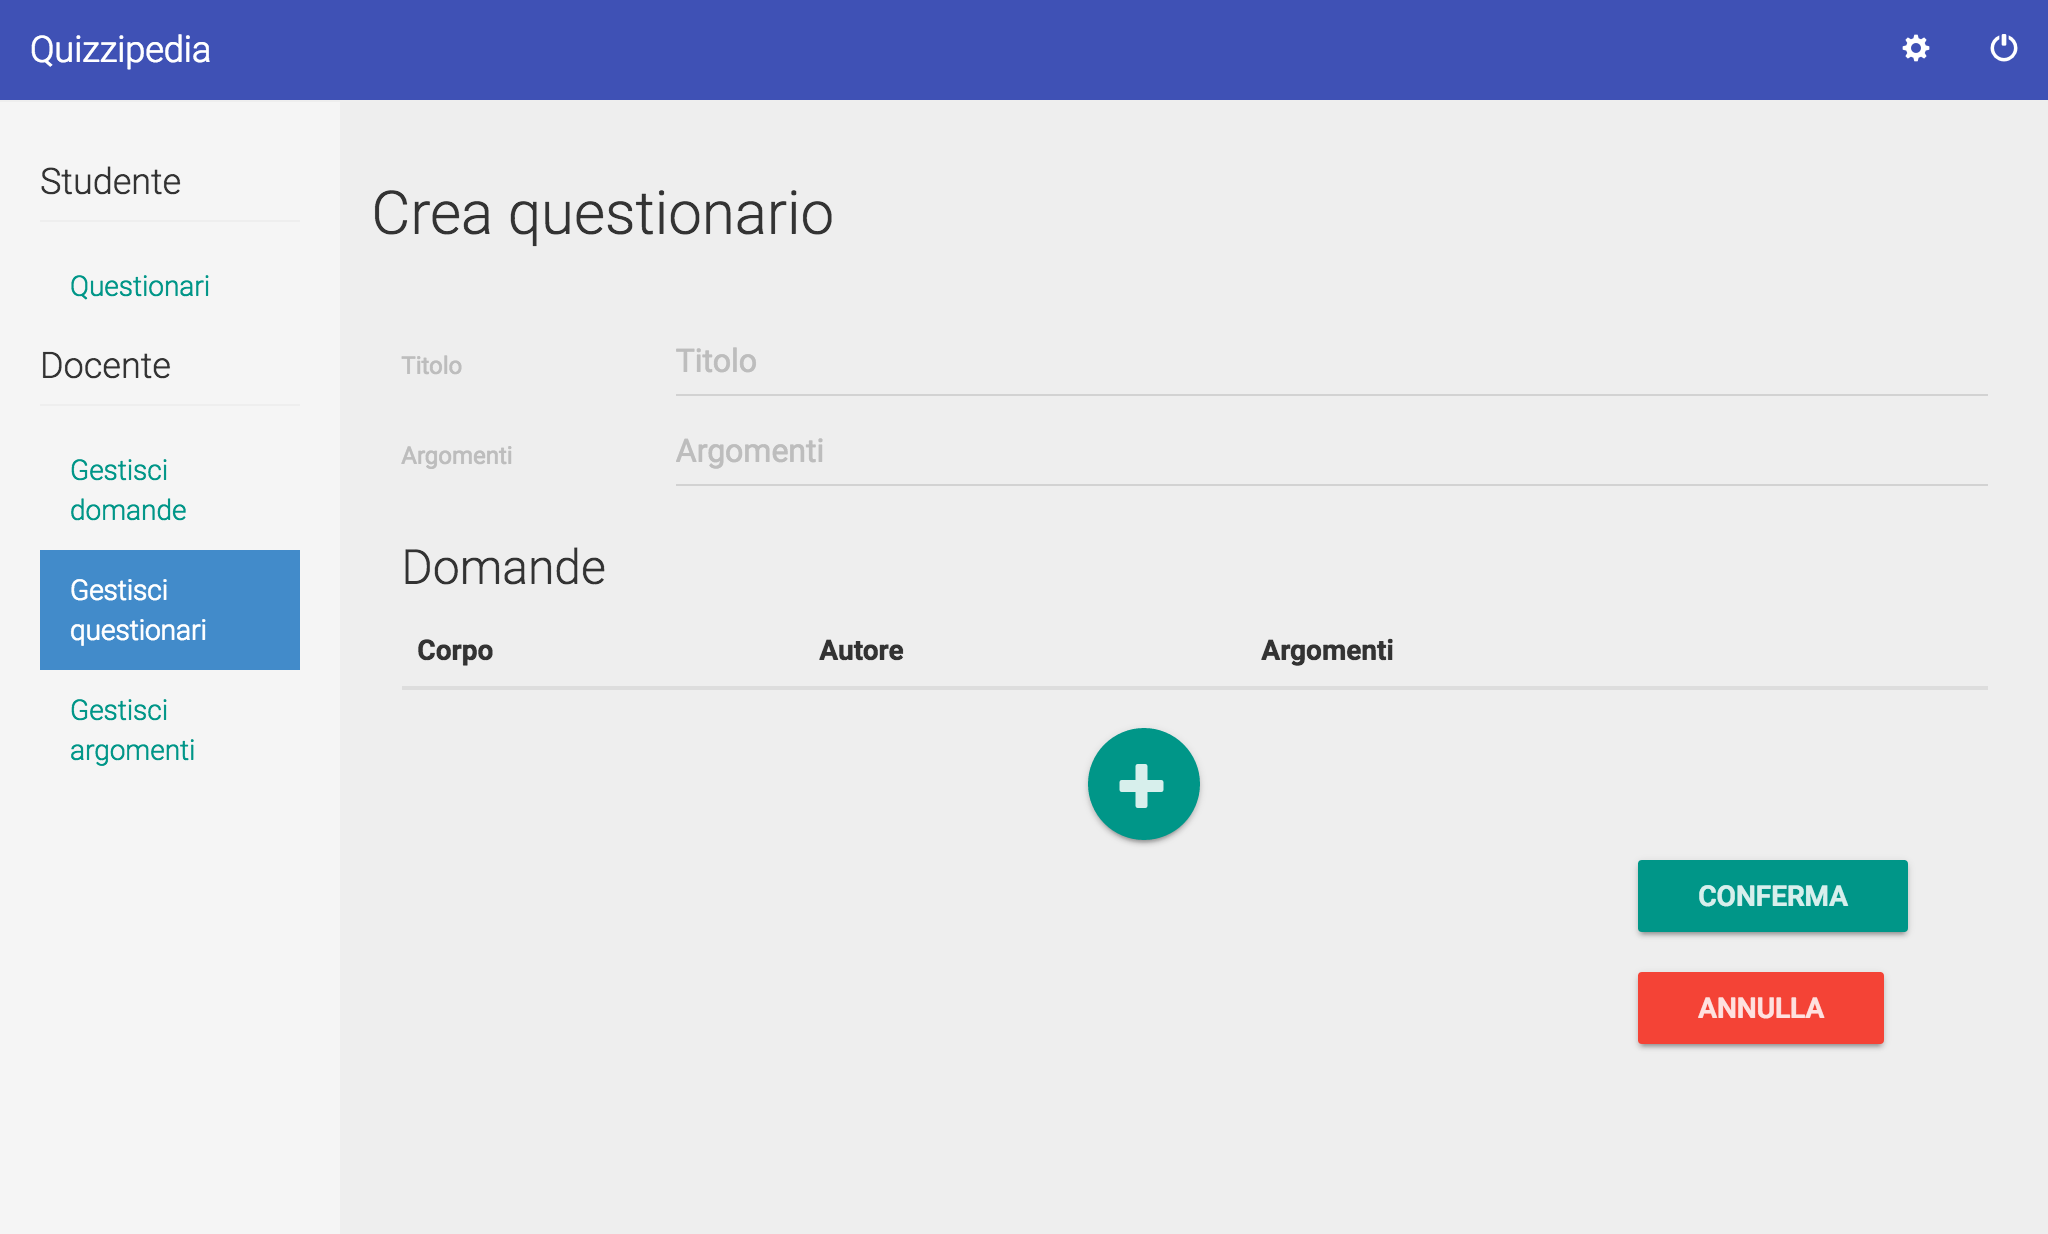
\includegraphics[width=1.0\linewidth]{../img/screenshot/creazioneQuestionario.png}
			\caption{}
			\label{Creazione questionario}
		\end{figure}
		
		\subsubsubsection{Modifica questionario}
		Per modificare un questionario è necessario selezionare il questionario che si desidera modificare. Si aprirà una schermata che permetterà di editare il titolo del questionario, di aggiungere o rimuovere domande e di aggiungere o rimuovere argomenti dal questionario corrente.
		Una volta terminata la modifica, selezionare la voce "submit" per rendere permanenti le modifiche effettuate. Per non salvare le modifiche effettuate selezionare "cacel".
			
		Nel caso la modifica non rispetti le regole per la definizione di un questionario, il sistema chiederà di modificare il questionario prima di salvare nuovamente.
		
		\begin{figure}[H]	
			\centering
			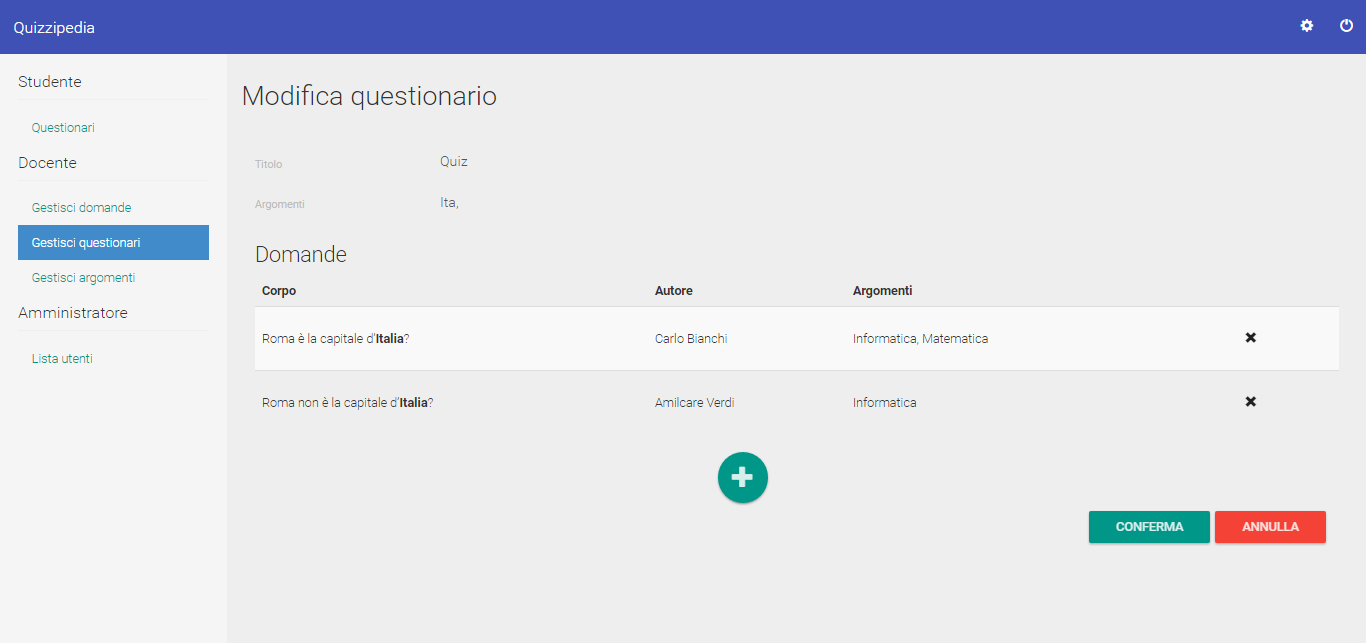
\includegraphics[width=1.0\linewidth]{../img/screenshot/modificaQuestionario.png}
			\caption{}
			\label{Modifica Questionario}
		\end{figure}
			
		\subsubsubsection{Eliminazione questionario}
		Per eliminare un questionario è necessario selezionare la voce "x" a fianco del questionario da eliminare. Prima di eliminare un questionario definitivamente, il sistema chiederà di confermare nuovamente l'eliminazione.
		Verrà aperta una finestra che chiederà di confermare o annullare l'eliminazione. Cliccando la voce "elimina", il questionario selezionato verrà eliminato irreversibilmente. Cliccando la voce "annulla", il procedimento di eliminazione verrà interrotto e il questionario non verrà eliminato.
		
		\begin{figure}[H]	
			\centering
			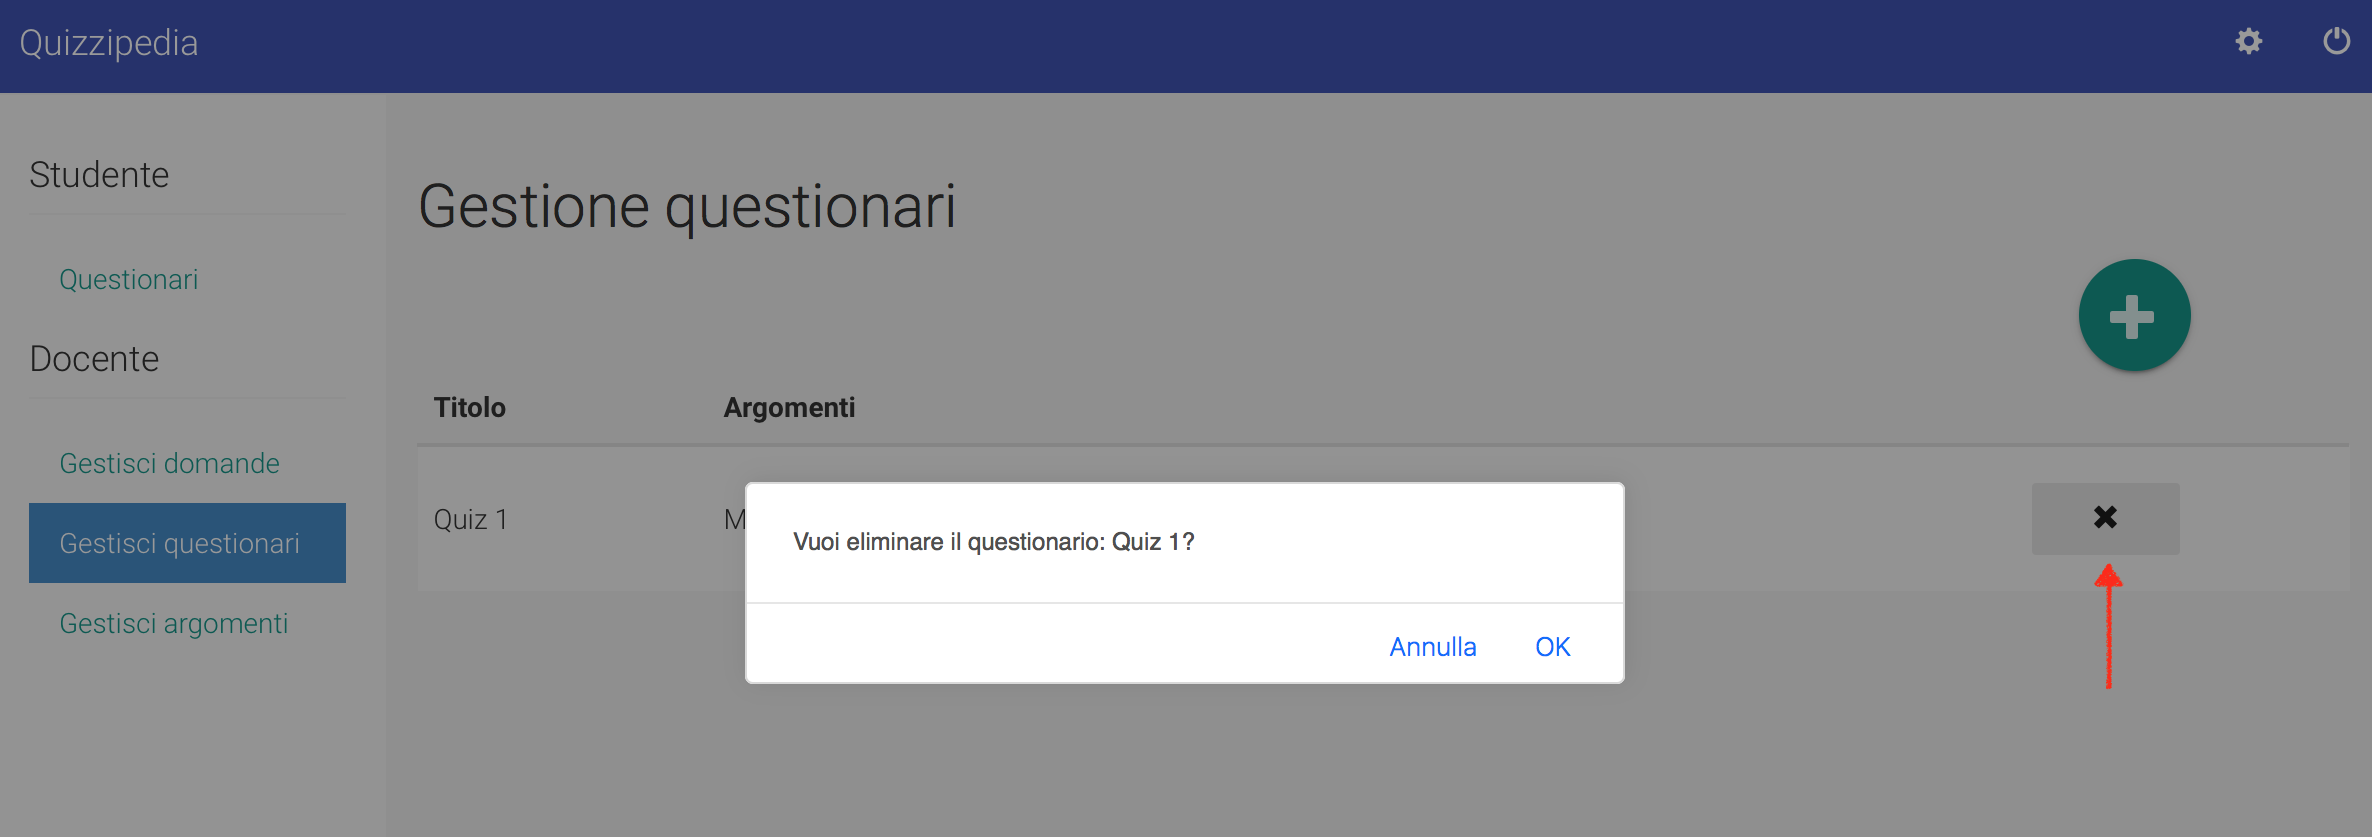
\includegraphics[width=0.8\linewidth]{../img/screenshot/eliminaQuestionario.png}
			\caption{}
			\label{Elimina questionario}
		\end{figure}
		
		\section{Amministratore}
		Un profilo amministratore ha accesso a tutte le funzionalità di docente e studente.
		Inoltre offre funzionalità aggiuntive quali:
		\begin{itemize}
			\item la possibilità di promuovere uno studente a ruolo di docente;
			\item la possibilità di degradare un docente a ruolo di studente;
			\item la possibilità di rimuovere un docente o uno studente dal sistema.
		\end{itemize}
		\subsection{Funzionalità docente}
		
		\subsubsection{Lista utenti e filtri}
		Per accedere alla pagina di gestione degli utenti è necessario selezionare la voce "Lista utenti" del menù amministratore.
		\begin{figure}[H]
			\centering
			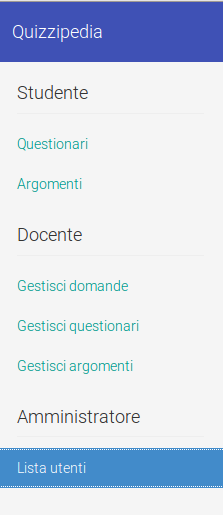
\includegraphics[width=0.2\linewidth]{../img/screenshot/usersListMenu.png}
			\caption{}
			\label{Lista utenti}
		\end{figure}
        Dalla schermata "Lista Utenti" è possibile filtrare gli utenti presenti nel sistema per ruolo cliccando sulla relativa opzione del filtro "Mostra".
		\begin{figure}[H]
			
			\centering
			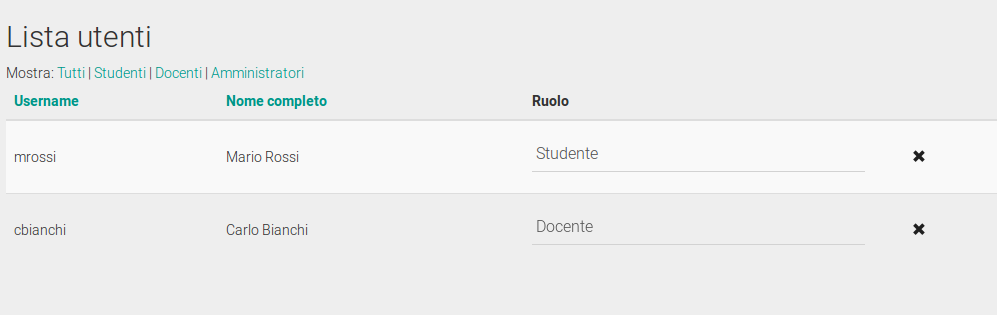
\includegraphics[width=1.0\linewidth]{../img/screenshot/usersListCrop.png}
			\caption{}
			\label{Lista utenti}
		\end{figure}
	
	\subsubsection{Gestione docenti}
	Selezionando un utente dalla lista utenti, un amministratore può effettuare alcune operazioni quali  il cambiamento di ruolo di un utente selezionato o la sua eliminazione dal sistema.
		
	\subsubsubsection{Eliminazione utente}
	L'amministratore per eliminare un utente dal sistema, dovrà cliccare sulla "x" che si trova infondo a destra  in corrispondenza del nome selezionato. Prima di eliminare definitivamente un utente, il sistema chiederà se confermare o annullare l'eliminazione. Cliccando sulla voce "elimina", l'utente selezionato verrà eliminato in maniera irreversibile. Cliccando su "annulla", il procedimento di eliminazione verrà unterrotto e l'utente non verrà eliminato.
		\begin{figure}[H]
			\centering
			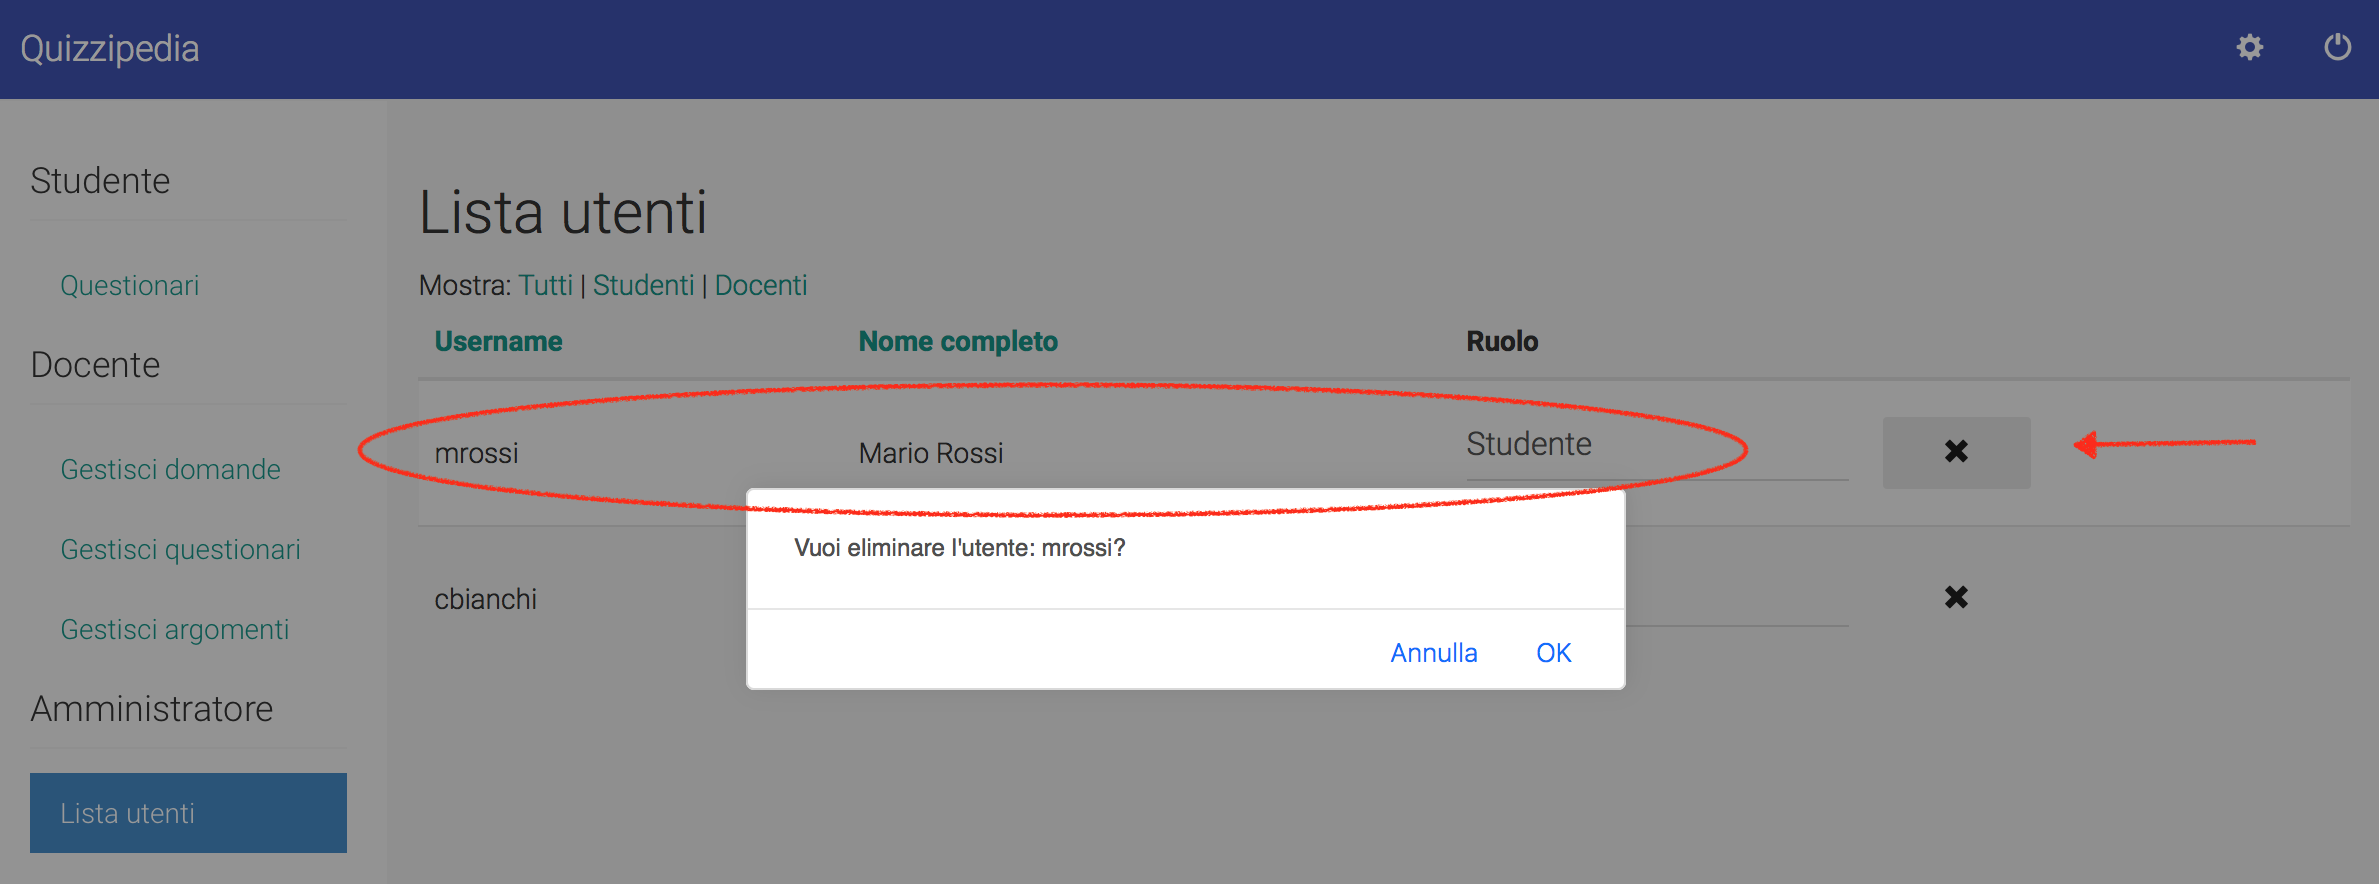
\includegraphics[width=1\linewidth]{../img/screenshot/rimozioneUtente.png}
			\caption{}
			\label{Rimozione utente}
		\end{figure}
	\subsubsubsection{Promozione a ruolo docente}
	Dalla lista utenti l'amministratore per promuovere lo studente a docente dovrà cliccare in corrispondenza del ruolo dello studente selezionato. In questo modo comparirà una combobox e tra le varie voci scegliere "docente". L'opzione con la spunta coinciderà con il ruolo che l'utente possiede in questo momento, mentre la parte evidenziata coincide con il ruolo che si vuole avere dopo la modifica.
	
	\begin{figure}[H]
		\centering
		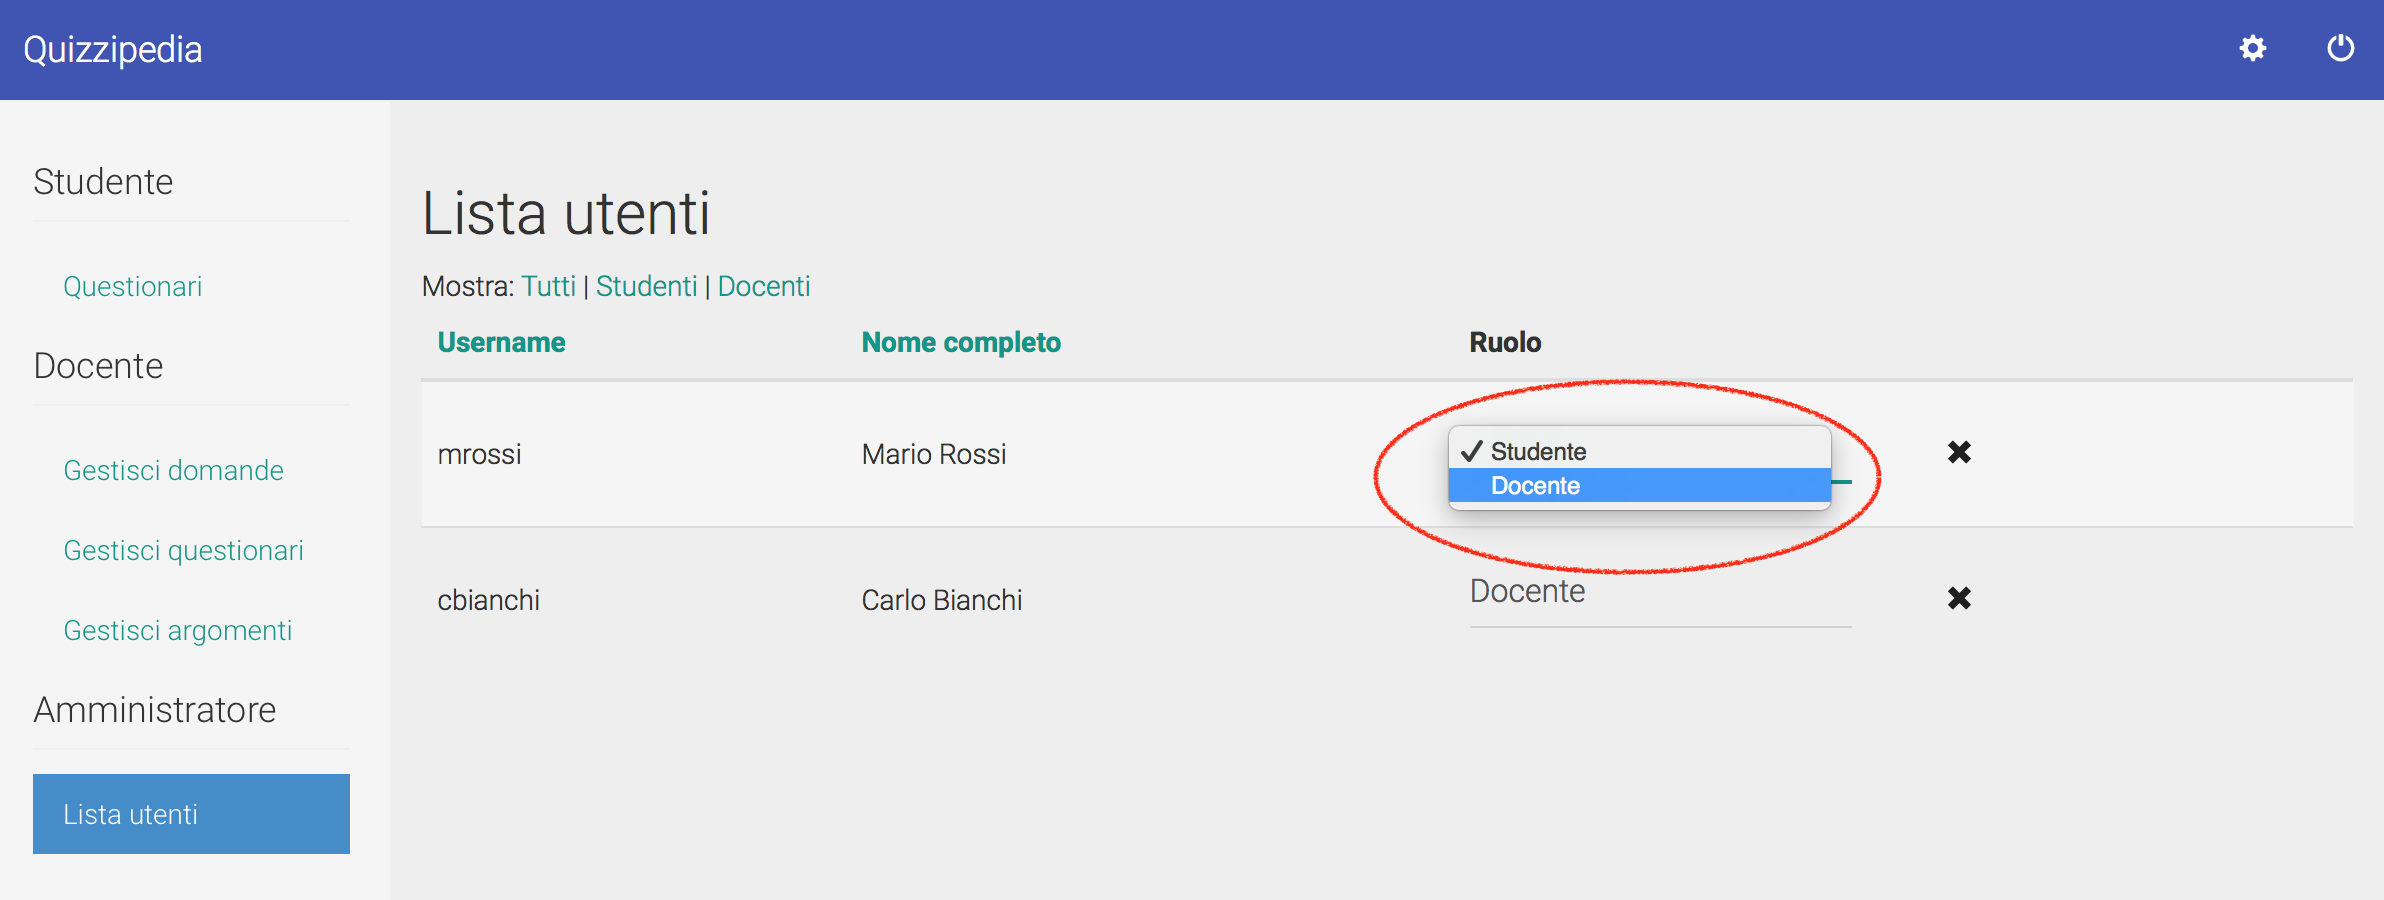
\includegraphics[width=1\linewidth]{../img/screenshot/cambioRuoloStudDoc.png}
		\caption{}
		\label{Promozione a ruolo docente}
	\end{figure}
	
	\subsubsubsection{Rimozione da ruolo docente}
	Per pimuove un docente dal suo incarico l'amministratore dovrà cliccare in corrispondenza del ruolo del docente  che si vuole degradare. In questo modo comparirà una combobox e tra le varie voci scegliere su "studente".
	L'opzione con la spunta coinciderà con il ruolo che l'utente possiede in questo momento, mentre la parte evidenziata coincide con il ruolo che si vuole avere dopo la modifica.
	
		\begin{figure}[H]
			\centering
			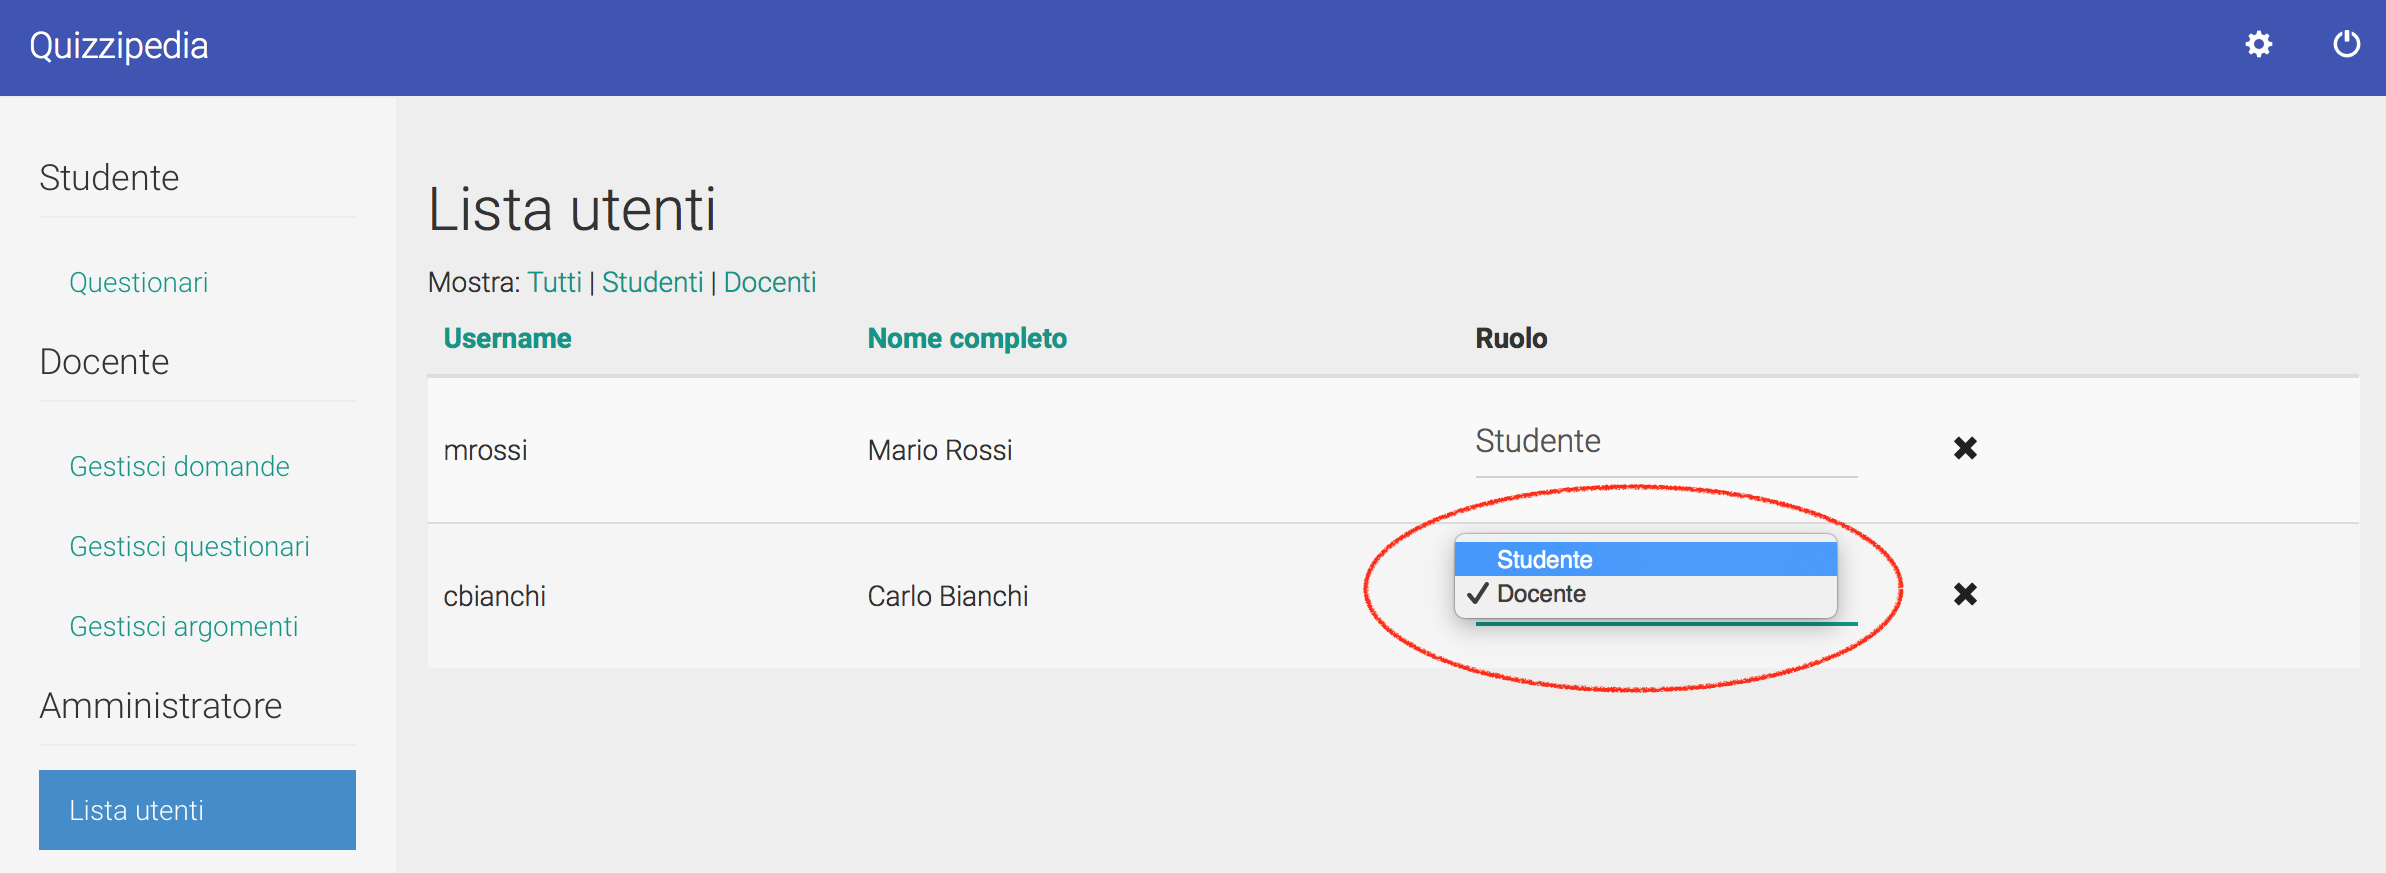
\includegraphics[width=1\linewidth]{../img/screenshot/cambioRuoloDocStud.png}
			\caption{}
			\label{Rimozione da ruolo docente}
		\end{figure}
	
	\section{Proprietario} 
	Un profilo proprietario ha accesso a tutte le funzionalità di docente, studente e amministratore.
	Inoltre offre funzionalità aggiuntive quali:
	\begin{itemize}
		\item la possibilità di promuovere uno utente (docente/studente) a ruolo di amministratore;
		\item la possibilità di degradare un amministratore a ruolo di studente o docente;
		\item la possibilità di rimuovere un amministratore dal sistema.
	\end{itemize}
	\subsection{Funzionalità proprietario}
	
	\subsubsection{Gestione  amministratori}
	Selezionando un utente dalla lista utenti, il proprietario può eseguire tutte le opeazioni descritte nella sezione amministratore con la possibilità di promuovere un qualsiasi utente ad amministratore o eventualmente degradare un amministratore o a docente o a studente.
	
	\subsubsubsection{Promozione ad amministratore}
	Dalla lista utenti il proprietario per promuovere un utente ad amministratore dovrà cliccare in corrispondenza del ruolo che attualmente tale utente riveste. In questo modo comparirà una combobox e scegliere su "amministratore". L'opzione con la spunta coinciderà con il ruolo che l'utente possiede in questo momento, mentre la parte evidenziata coincide con il ruolo che si vuole avere dopo la modifica.
	
		\begin{figure}[H]
			\centering
			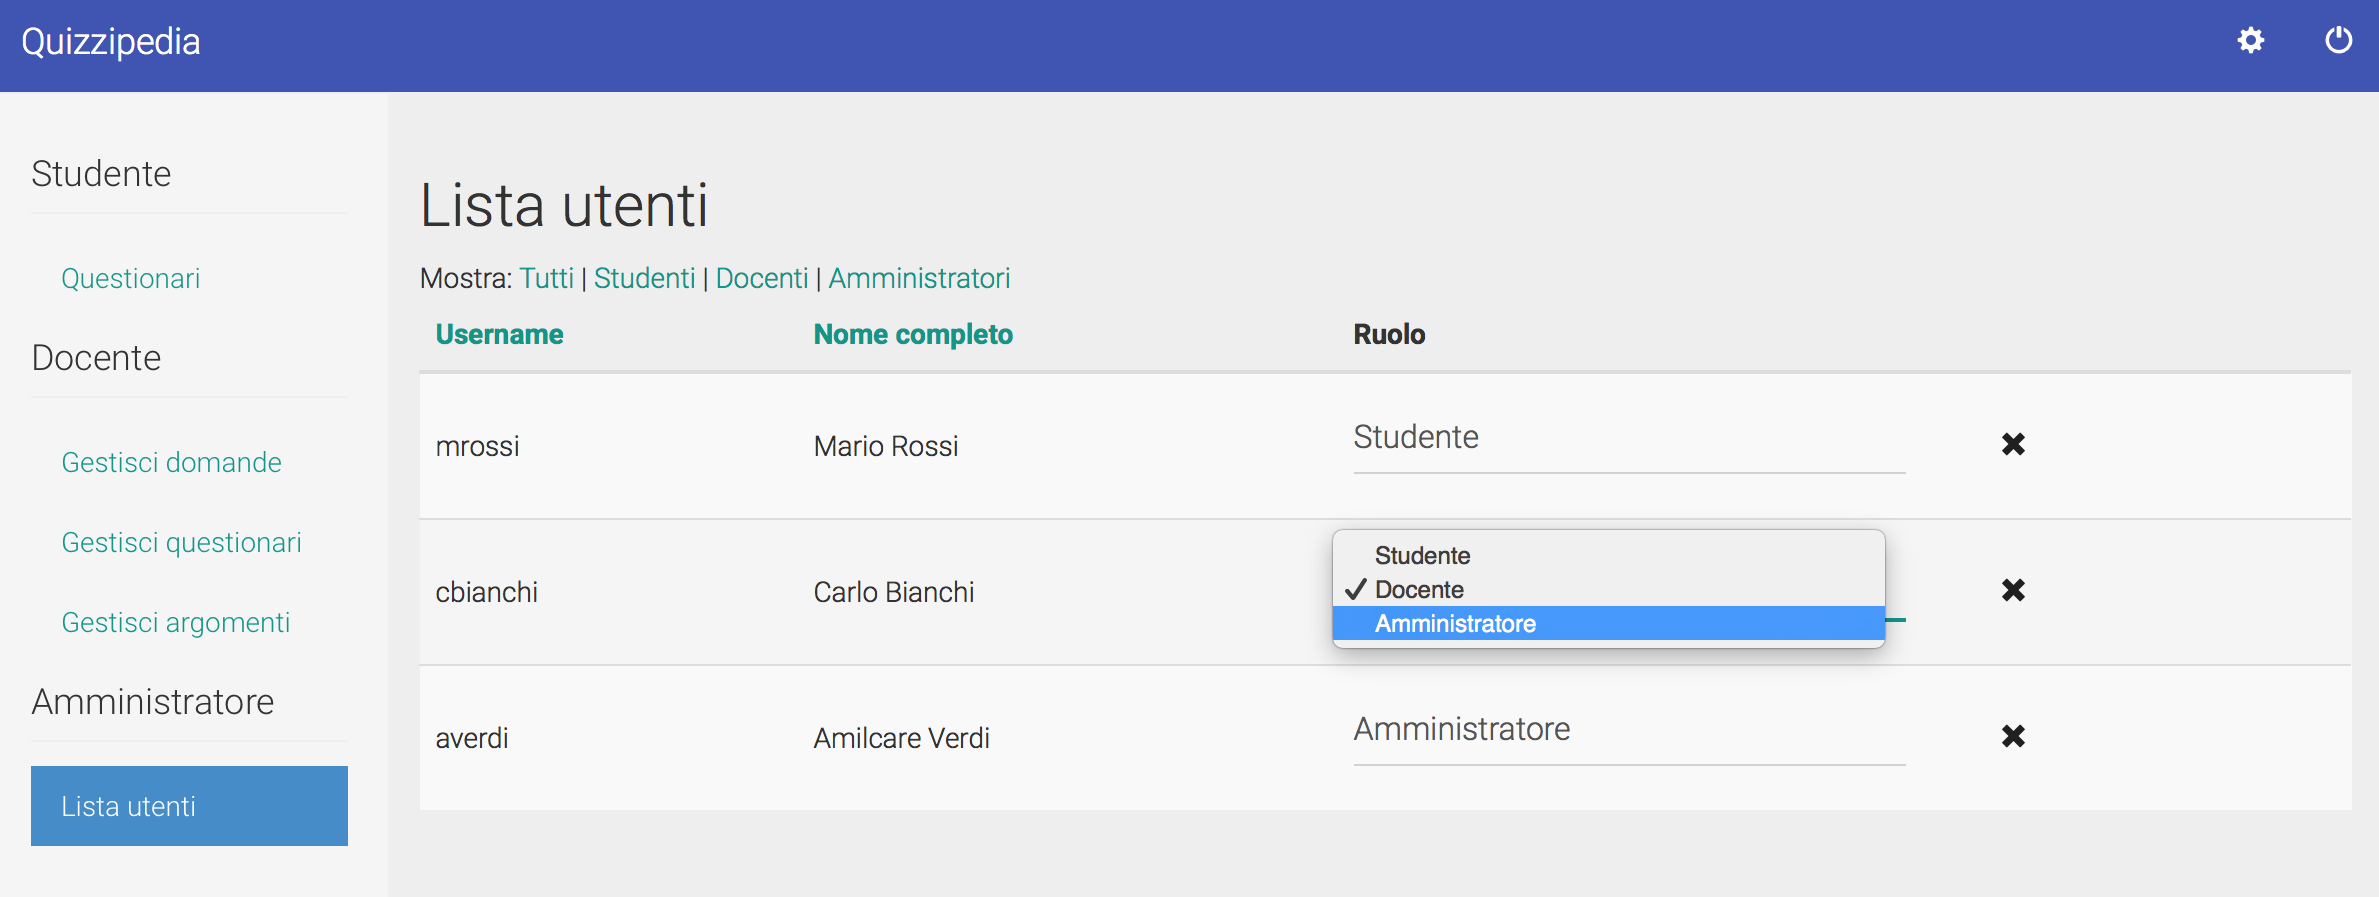
\includegraphics[width=1\linewidth]{../img/screenshot/cambioRuoloDocAmm.png}
			\caption{}
			\label{Promozione ad amministratore}
		\end{figure}
	
	\subsubsubsection{Rimozione dal ruolo amministratore}
	Per pimuove un amministratore dal suo incarico il proprietario dovrà cliccare in corrispondenza del ruolo dell'amministratore che si vuole degradare. In questo modo comparirà una combobox e scegliere su "studente" o "docente". L'opzione con la spunta coinciderà con il ruolo che l'utente possiede in questo momento, mentre la parte evidenziata coincide con il ruolo che si vuole avere dopo la modifica.
	
		\begin{figure}[H]
			\centering
			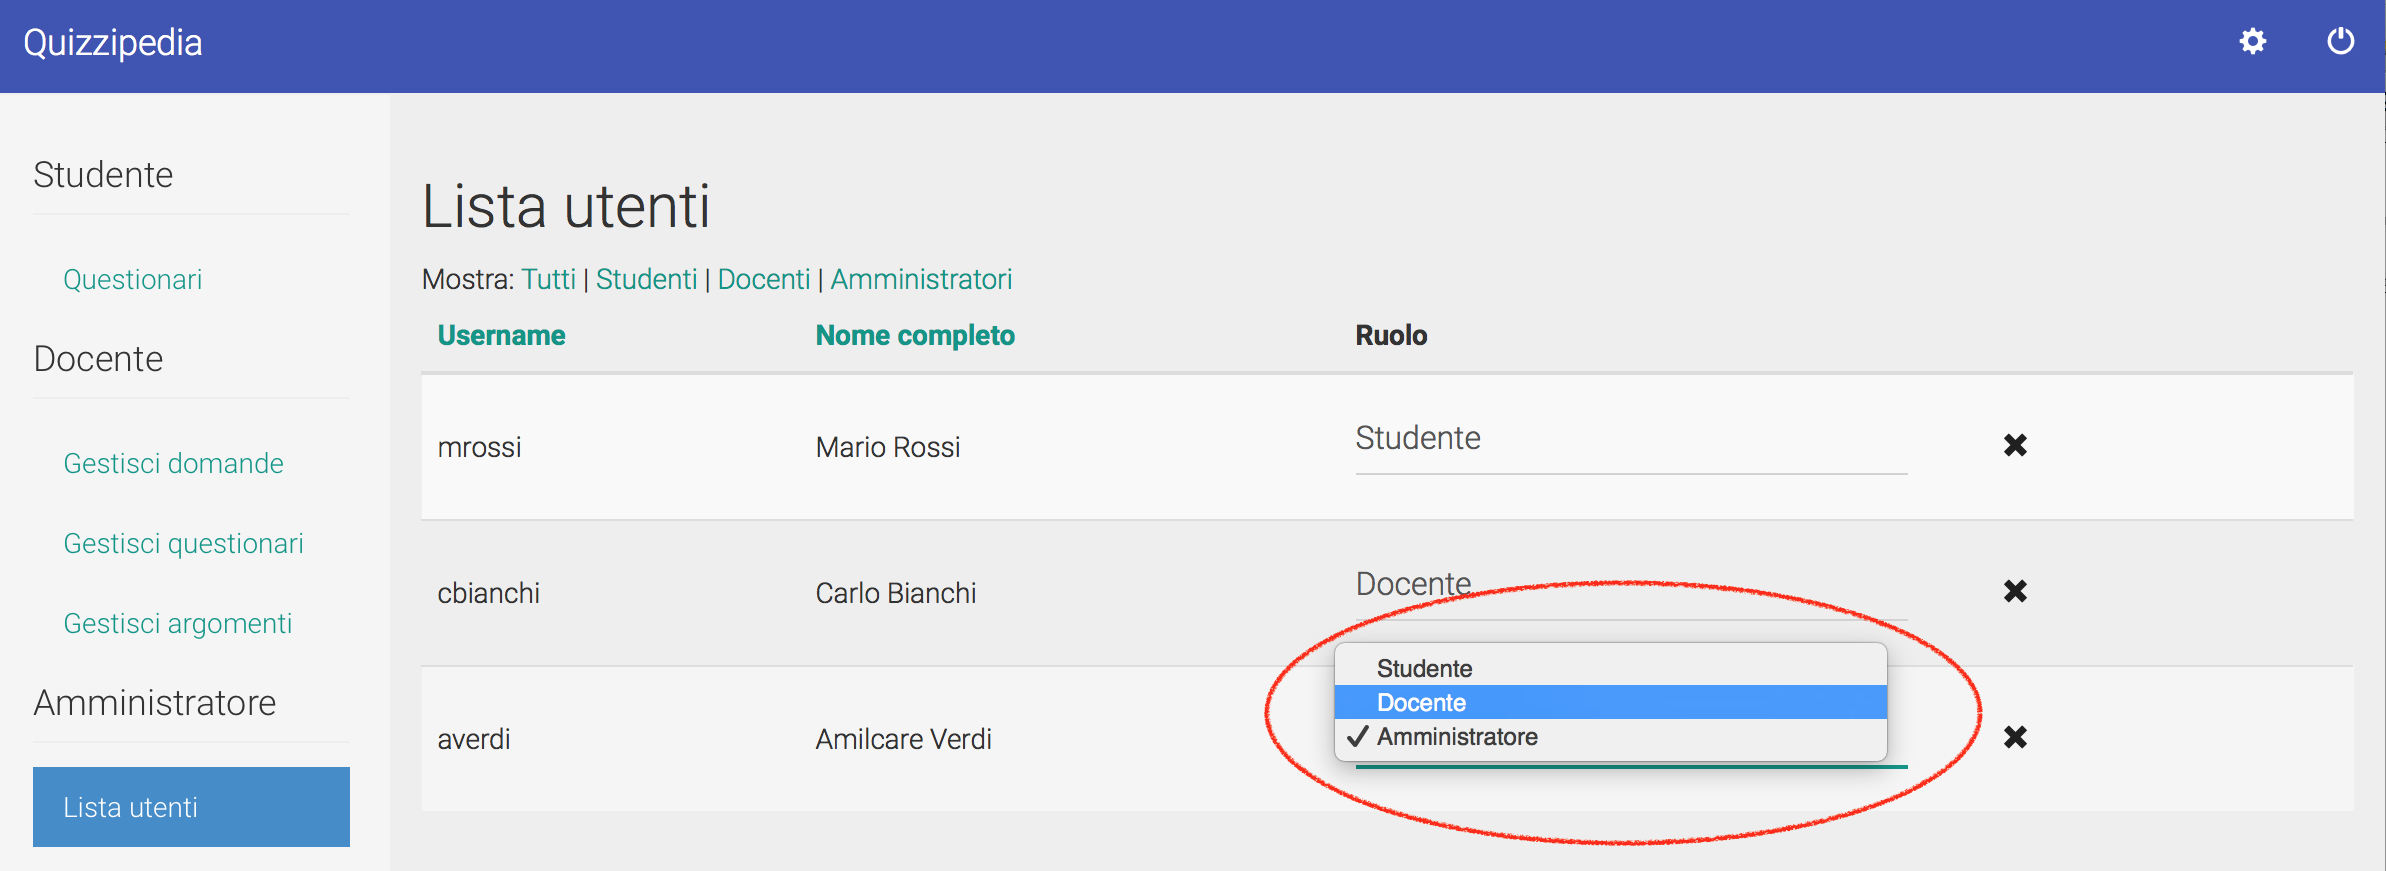
\includegraphics[width=1\linewidth]{../img/screenshot/cambioRuoloAmmDoc.png}
			\caption{}
			\label{Rimozione dal ruolo amministratore}
		\end{figure}
	
	\subsubsubsection{Rimozione amministratore}
	L'amministratore per eliminare un utente dal sistema, dovrà cliccare sulla "x" che si trova infondo a destra  in corrispondenza dell'amministratore selezionato. Prima di eliminare definitivamente un'amministratore, il sistema chiederà se confermare o annullare l'eliminazione. Cliccando sulla voce "elimina", l'amministratore selezionato verrà eliminato in maniera irreversibile. Cliccando su "annulla", il procedimento di eliminazione verrà unterrotto e l'amministratore non verrà eliminato.
	
		\begin{figure}[H]
			\centering
			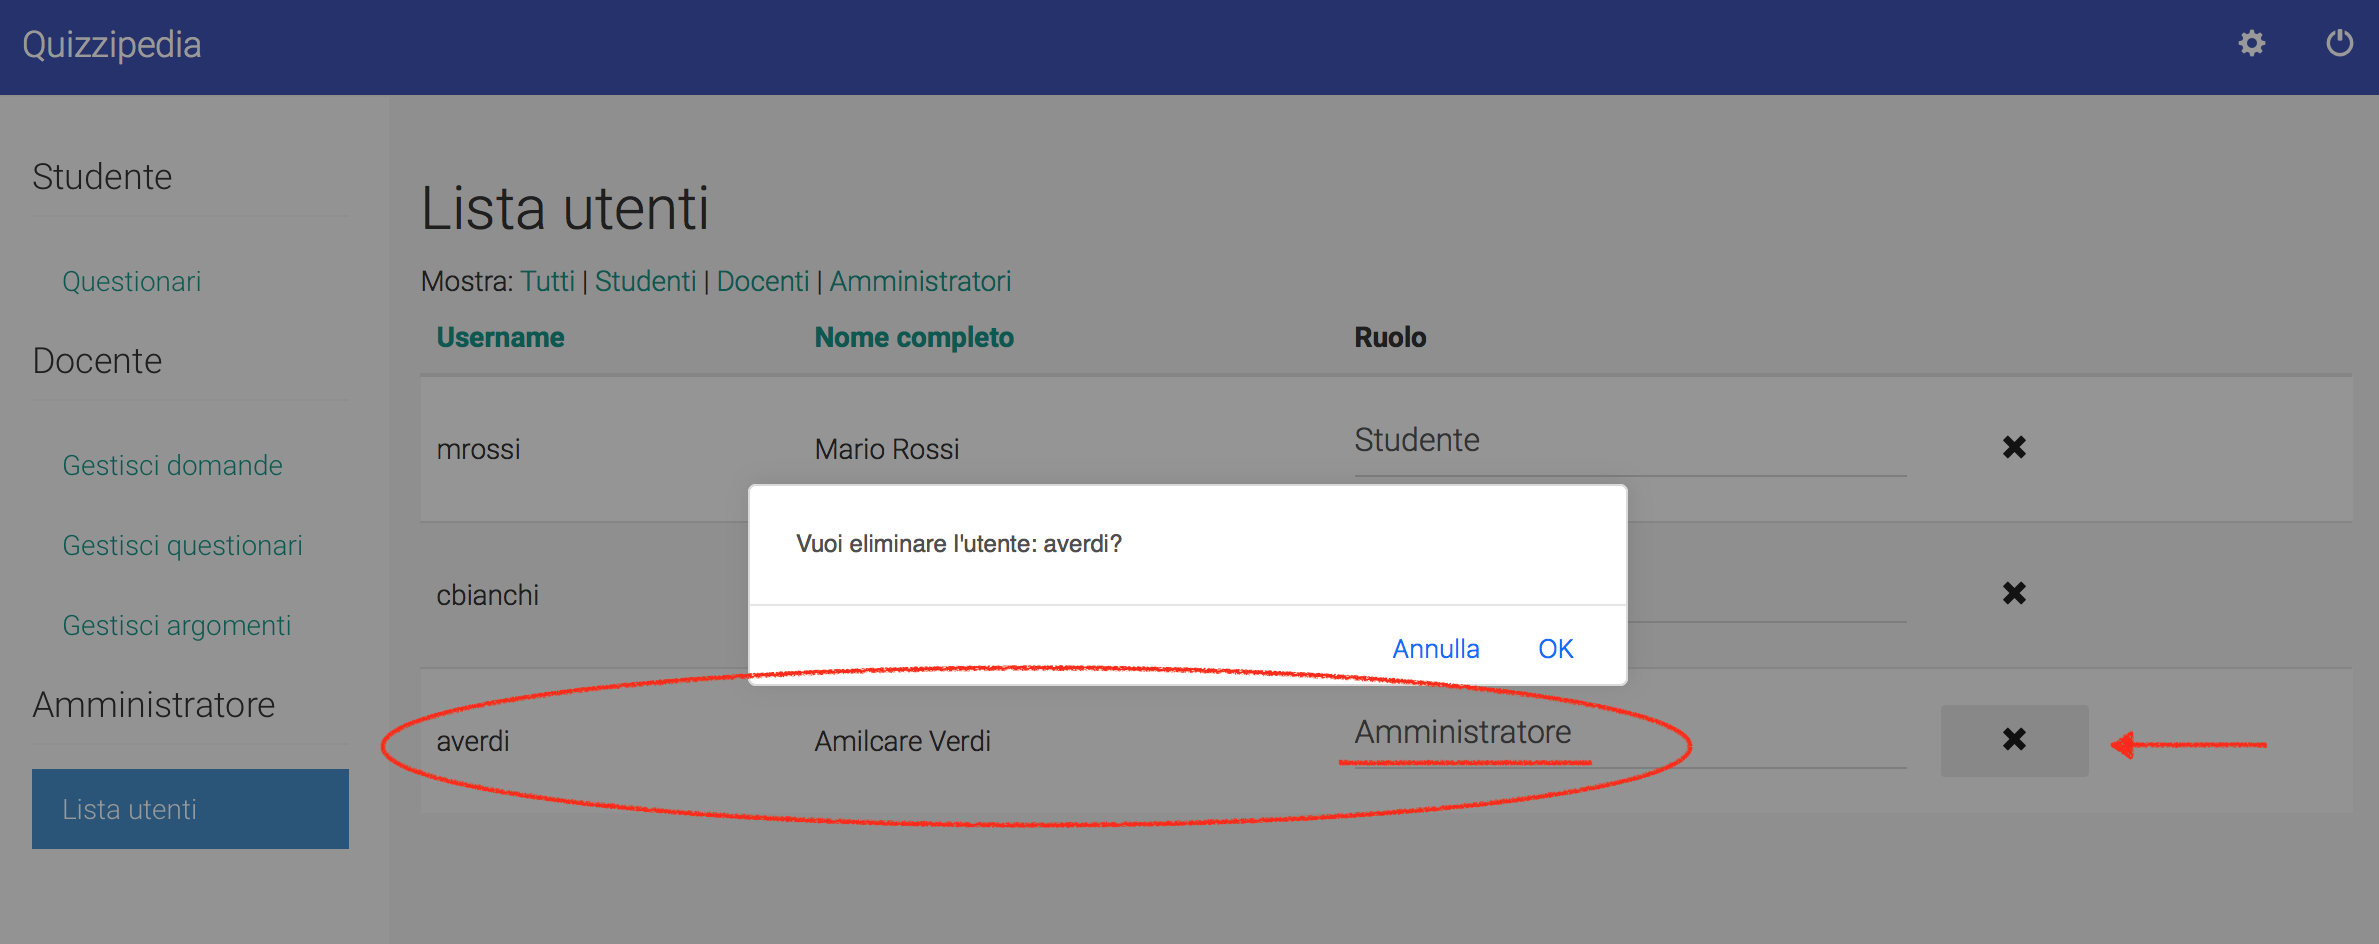
\includegraphics[width=1\linewidth]{../img/screenshot/rimozioneAmministratore.png}
			\caption{}
			\label{Rimozione di un amministratore dal sistema}
		\end{figure}
	
	\section{Definizione QML}
	Il QML (Question Markup Language) è il linguaggio per definire la struttura di una domanda. La struttura comincia con la definizione del tipo di domanda e continua con una parte variabile a seconda del tipo.\\
	\begin{verbatim}
	<Tipo di domanda>
	parte variabile
	\end{verbatim}
		
	 I tipi supportati sono:
	\begin{verbatim}
		\item Domanda Vero/Falso
		\item Domanda a scelta multipla
	\end{verbatim}
	Per i testi delle domande e delle risposte si utilizza il parsing markdown. Per una guida su questo linguaggio si rimanda a: \url{https://github.com/adam-p/markdown-here/wiki/Markdown-Cheatsheet}. In questo modo, per esempio è possibile aggiungere formattazione al testo, tabelle e immagini, queste ultime tramite il comando\\
	 \texttt{![alt text](https://flic.kr/p/GxRmqq "Immagine1")}\\
		
	\subsection{Domanda Vero/Falso}
	\paragraph{Domanda vera}
	\begin{verbatim}
	<TF T>
	Domanda_in_markdown
	\end{verbatim}
	\paragraph{Domanda falsa}
	\begin{verbatim}
	<TF F>
	Domanda_in_markdown
	\end{verbatim}
	\paragraph{Esempio}
	\begin{verbatim}
	<TF T>
	Roma e' la capitale d'**Italia**?
	\end{verbatim}
	
	\subsection{Domanda a scelta multipla}
	\begin{verbatim}
	<MultipleChoice>
	Domanda_in_markdown
	[answers]
	[]Risposta_sbagliata
	[*]Risposta_giusta
	[]Risposta_sbagliata
	\end{verbatim}
	\paragraph{Esempio}
	\begin{verbatim}
	<MultipleChoice>
	Qual è la capitale d'**Italia**?
	[answers]
	[] Berlino
	[*] Roma
	[] Padova
	\end{verbatim}
	
	
\end{document}
